\documentclass[12pt,a4paper,oneside]{report}
\usepackage[T1]{fontenc}
\usepackage{mathptmx}
\usepackage[left=30mm,right=25mm,top=25mm,bottom=25mm]{geometry}

\usepackage{amsmath,amssymb,amsfonts}
\usepackage{titlesec}
\usepackage{fancyhdr}
\setlength{\headheight}{30pt}
\setlength{\headsep}{12pt}

\usepackage{graphicx,array,longtable,pdflscape,setspace}
\usepackage{booktabs,multirow}
\usepackage{tikz}
\usetikzlibrary{shapes.geometric,arrows.meta,positioning,calc,fit,backgrounds}
\usepackage{algorithm}
\usepackage{algpseudocode}
\usepackage{listings}
\usepackage{xcolor}
\usepackage[hidelinks]{hyperref}
\onehalfspacing
\setlength{\parindent}{0pt}
\setlength{\parskip}{4pt}
\setcounter{tocdepth}{2}
\renewcommand{\contentsname}{Table of Contents}
\newcommand{\institutionlogo}[1]{\IfFileExists{amrita-logo.png}{
\includegraphics[width=#1]{amrita-logo.png}}{\fbox{\parbox{#1}{\centering \textbf{Amrita Vishwa Vidyapeetham}\\[4pt]\small Place amrita-logo.png beside this file}}}}

% Project Title defined here
\newcommand{\ProjectTitle}{AppPoet: Multimodal Android Malware Detection via Behavior-Aware Semantic Abstraction and Structural Graph Learning}

\fancypagestyle{project}{%
  \fancyhf{}
  \fancyhead[C]{\parbox{\textwidth}{\centering\small\nouppercase{\ProjectTitle}}}
  \fancyfoot[C]{\thepage}
  \renewcommand{\headrulewidth}{0.4pt}
}

% Preliminary pages show only a page number.
\fancypagestyle{plain}{%
  \fancyhf{}
  \fancyfoot[C]{\thepage}
  \renewcommand{\headrulewidth}{0pt}
}

\newcommand{\EnableProjectHeaders}{%
  \pagestyle{project}%
  % report uses plain style on chapter-opening pages.
  \fancypagestyle{plain}{%
    \fancyhf{}
    \fancyhead[C]{\parbox{\textwidth}{\centering\small\nouppercase{\ProjectTitle}}}
    \fancyfoot[C]{\thepage}
    \renewcommand{\headrulewidth}{0.4pt}
  }%
}

\titlespacing*{\chapter}{0pt}{0pt}{16pt}
\titlespacing*{\section}{0pt}{10pt}{4pt}
\titlespacing*{\subsection}{0pt}{8pt}{3pt}
\titlespacing*{\subsubsection}{0pt}{6pt}{3pt}
\raggedbottom

% Listings configuration for Appendix
\definecolor{codegreen}{rgb}{0,0.6,0}
\definecolor{codegray}{rgb}{0.5,0.5,0.5}
\definecolor{codepurple}{rgb}{0.58,0,0.82}
\definecolor{backcolour}{rgb}{0.97,0.97,0.97}

\lstdefinestyle{pythonstyle}{
    backgroundcolor=\color{backcolour},   
    commentstyle=\color{codegreen},
    keywordstyle=\color{magenta},
    numberstyle=\tiny\color{codegray},
    stringstyle=\color{codepurple},
    basicstyle=\ttfamily\footnotesize,
    breakatwhitespace=false,         
    breaklines=true,                 
    captionpos=b,                    
    keepspaces=true,                 
    numbers=left,                    
    numbersep=5pt,                  
    showspaces=false,                
    showstringspaces=false,
    showtabs=false,                  
    tabsize=2
}
\lstset{style=pythonstyle}

\begin{document}
\pagestyle{empty}

{\centering \Large\bfseries \ProjectTitle{}\par}
\vspace{0.5cm}
{\centering Project report submitted in partial fulfilment of the requirements for the award of the degree of\par}
\vspace{0.5cm}
{\centering \textbf{BACHELOR OF TECHNOLOGY}\par}
{\centering in\par}
{\centering \textbf{COMPUTER SCIENCE AND ENGINEERING}\par}
\vspace{0.5cm}
{\centering Submitted by\par}
\vspace{0.5cm}
{\centering \fontsize{14}{18}\selectfont
\textbf{B. Ravindranath} \quad AM.SC.U4CSE23019\par}

{\centering \fontsize{14}{18}\selectfont
\textbf{M. Subba Rao} \quad AM.SC.U4CSE23050\par}

{\centering \fontsize{14}{18}\selectfont
\textbf{A. Arjun} \quad AM.SC.U4CSE23011\par}

{\centering \fontsize{14}{18}\selectfont
\textbf{R. Jitin Sai} \quad AM.SC.U4CSE23072\par}
\vspace{0.5cm}
{\centering \fontsize{14}{18}\selectfont
Under the guidance of\par
\textbf{Dr. Deepthi L. R.}\par}
\vspace{0.5cm}
{\centering \institutionlogo{4.5in}\par}
\vspace{0.5cm}
{\centering \textbf{AMRITA SCHOOL OF COMPUTING}\par}
{\centering \textbf{AMRITA VISHWA VIDYAPEETHAM}\par}
{\centering \textbf{AMRITAPURI CAMPUS}\par}
{\centering \textbf{KOLLAM 690525}\par}
{\centering \textbf{NOVEMBER 2026}\par}

\clearpage
{\centering \institutionlogo{3.7in}\par}
{\centering \textbf{DEPARTMENT OF COMPUTER SCIENCE AND ENGINEERING}\par}
{\centering Amrita School of Computing, Amritapuri Campus\par}
\vspace{0.5cm}
{\centering \Large\bfseries BONAFIDE CERTIFICATE\par}
\vspace{0.5cm}
This is to certify that the project report entitled ``\ProjectTitle{}'', submitted by \textbf{B. Ravindranath} (AM.SC.U4CSE23019), \textbf{M. Subba Rao} (AM.SC.U4CSE23050), \textbf{A. Arjun} (AM.SC.U4CSE23011) and \textbf{R. Jitin Sai} (AM.SC.U4CSE23072), in partial fulfilment of the requirements for the award of the degree of Bachelor of Technology in Computer Science and Engineering at Amrita Vishwa Vidyapeetham, is a bonafide record of the work carried out by them under my guidance and supervision at Amrita School of Computing, Amritapuri, during Semester 7 of the academic year 2026 - 2027.

\vspace{1cm}
\begin{tabular}{p{.46\textwidth}p{.46\textwidth}} 
\textbf{Dr. Deepthi L. R.} & \textbf{Dr. Aswathy Mohan} \\ 
Project Guide & Project Coordinator \\ 
Signature \hrulefill & Signature \hrulefill \\[24pt] 
\textbf{Dr. Swaminathan} &  \\ 
Chairperson, CSE & Reviewers \\ 
Signature \hrulefill & Signature \hrulefill 
\end{tabular}
\\
\\ 
\\ Place: Amritapuri\\
Date: 
\clearpage
\thispagestyle{empty}

{\centering
\institutionlogo{3.7in}\par
\vspace{0.4cm}
\textbf{DEPARTMENT OF COMPUTER SCIENCE AND ENGINEERING}\par
Amrita School of Computing, Amritapuri Campus\par
\vspace{0.6cm}
{\Large\bfseries DECLARATION\par}
}

\vspace{0.5cm}

\noindent
We, \textbf{B. Ravindranath} (AM.SC.U4CSE23019),
\textbf{M. Subba Rao} (AM.SC.U4CSE23050),
\textbf{A. Arjun} (AM.SC.U4CSE23011) and
\textbf{R. Jitin Sai} (AM.SC.U4CSE23072),
hereby declare that the project entitled
``\ProjectTitle{}'' is a record of our original work
carried out under the guidance of \textbf{Dr. Deepthi L. R.},
Department of Computer Science and Engineering,
Amrita Vishwa Vidyapeetham, Amritapuri.
To the best of our knowledge, this work has not formed the
basis for the award of any degree, diploma, fellowship or
similar qualification to any candidate at any university.
All sources and contributions of others have been
appropriately acknowledged.

\vspace{0.5cm}

\noindent
Place: Amritapuri\\
Date: 

\vspace{0.7cm}

\noindent
\begin{tabular}{@{}p{0.60\textwidth}p{0.34\textwidth}@{}}
\textbf{Student details} & \textbf{Signature of the student} \\[14pt]

\textbf{B. Ravindranath}\newline
AM.SC.U4CSE23019
& \rule{0.30\textwidth}{0.4pt} \\[18pt]

\textbf{M. Subba Rao}\newline
AM.SC.U4CSE23050
& \rule{0.30\textwidth}{0.4pt} \\[18pt]

\textbf{A. Arjun}\newline
AM.SC.U4CSE23011
& \rule{0.30\textwidth}{0.4pt} \\[18pt]

\textbf{R. Jitin Sai}\newline
AM.SC.U4CSE23072
& \rule{0.30\textwidth}{0.4pt}
\end{tabular}

\vspace{0.8cm}

\noindent
\textbf{Project Guide:} Dr. Deepthi L. R.

\vspace{0.5cm}

\noindent
\textbf{Signature of the Project Guide:}
\rule{4cm}{0.4pt}

\clearpage
\pagenumbering{roman}
\pagestyle{plain}

\phantomsection
\addcontentsline{toc}{chapter}{Acknowledgement}
{\centering \Large\bfseries ACKNOWLEDGEMENT\par}
\vspace{0.5cm}
We express our deepest gratitude to our project guide, \textbf{Dr. Deepthi L. R.}, Department of Computer Science and Engineering, for her invaluable supervision, technical insights, and continuous encouragement throughout this project. We also extend our sincere thanks to \textbf{Dr. Aswathy Mohan}, Project Coordinator, and \textbf{Dr. Swaminathan}, Chairperson of the Department of Computer Science and Engineering, for providing the necessary computing infrastructure, research facilities, and academic support. 

We acknowledge Amrita Vishwa Vidyapeetham for fostering a rigorous research-driven environment that enabled the successful conceptualization, implementation, and empirical validation of this work. Finally, we convey our heartfelt appreciation to our families and peers whose unwavering moral support and constructive feedback served as a constant source of inspiration throughout the duration of this capstone research endeavor.

\clearpage
\phantomsection
\addcontentsline{toc}{chapter}{Abstract}
{\centering \Large\bfseries ABSTRACT\par}
\vspace{0.5cm}
The exponential expansion of the Android mobile ecosystem has precipitated an unprecedented surge in sophisticated mobile malware. Modern adversarial campaigns routinely circumvent conventional static signature-based detection mechanisms through polymorphic mutations, dynamic reflection, string encryption, and control-flow obfuscation. To counteract these evasive strategies, this project proposes \textbf{AppPoet}, a novel multimodal deep learning framework that integrates \textbf{Behavior-Aware Semantic Abstraction} with \textbf{Structural Graph Learning}. 

The proposed architecture resolves the limitations of single-modality systems by capturing both the declared operational intent and the underlying execution topology of Android applications. The semantic analysis branch extracts manifest permissions, hardware features, broadcast receivers, background services, and invocation profiles across a curated catalog of the top 200 sensitive Android APIs across eight security-critical functional domains. A Large Language Model (LLM) processes these multifaceted static attributes to generate rich, coherent behavioral summaries across three distinct analytical views: (1) Declared Permission and Privilege View, (2) Component Architecture and Operational View, and (3) Sensitive API Execution View. These synthesized three-view summaries are subsequently handed off to a pre-trained \texttt{BAAI/bge-large-en-v1.5} sentence transformer to construct dense, contextualized 768-dimensional semantic embeddings. Concurrently, the structural branch constructs a directed Function Call Graph (FCG) from Dalvik bytecode. A DeepSAGE graph neural network, equipped with inductive neighborhood aggregators, is pre-trained via self-supervised Deep Graph Infomax (DGI) to maximize mutual information between localized sub-graph motifs and global topological representations, yielding a 256-dimensional structural embedding. 

To bridge the heterogeneous latent spaces, an asymmetric Multi-Head Cross-Attention mechanism is implemented, allowing structural call pathways to dynamically attend to declared semantic intents. Evaluated on a diverse benchmark corpus of 4,500 real-world applications (2,250 benign and 2,250 malicious samples across major malware families), AppPoet achieves an overall classification accuracy of \textbf{96.44\%}, an F1-score of \textbf{96.45\%}, a precision of \textbf{96.24\%}, a recall of \textbf{96.67\%}, and a Receiver Operating Characteristic Area Under Curve (ROC-AUC) of \textbf{0.9882}, outperforming unimodal semantic baselines ($90.89\%$) and structural graph baselines ($93.11\%$). The 512-dimensional fused representation is visualized via t-SNE projection, demonstrating clear cluster separability between benign applications and distinct malware families. 

Furthermore, this research directly contributes to the \textbf{United Nations Sustainable Development Goal 9 (SDG 9): Industry, Innovation, and Infrastructure}, specifically advancing Target 9.1 and Target 9.c by bolstering the cyber-resilience of digital telecommunications and mobile financial infrastructure against systemic zero-day threats.

\vspace{0.5cm}
\textbf{Keywords:} Android Malware Detection; Multimodal Deep Learning; Graph Neural Networks; GraphSAGE; Deep Graph Infomax; Natural Language Processing; Sentence Transformers; Cross-Attention Fusion; UN SDG 9.

\clearpage
\tableofcontents
\clearpage
\phantomsection
\addcontentsline{toc}{chapter}{List of Figures}
\listoffigures
\clearpage
\phantomsection
\addcontentsline{toc}{chapter}{List of Tables}
\listoftables
\clearpage
\pagenumbering{arabic}
\pagestyle{plain}
\EnableProjectHeaders

\chapter{Introduction}
\section{Background and Motivation}
Mobile computing has emerged as the definitive backbone of contemporary digital society. Smartphones powered by the Android operating system account for over 70\% of global mobile market share, supporting upwards of 3.9 billion active devices worldwide. Consequently, Android devices serve as primary repositories for sensitive personal data, corporate credentials, health telemetry, and financial payment gateways (such as Unified Payments Interface and mobile banking applications). This centralization of valuable digital assets has made the Android platform the foremost target of financially motivated cybercriminal syndicates, state-sponsored advanced persistent threat (APT) actors, and espionage groups.

The Android threat landscape has evolved dramatically over the past decade. Early malicious applications were predominantly simplistic SMS trojans (e.g., FakePlayer) that relied on overt, suspicious permission requests to bill victim accounts silently. Modern mobile malware, however, exhibits unprecedented operational sophistication. Prominent banking trojans (such as Anatsa, SharkBot, TeaBot, and FluBot), surveillance spyware (such as Pegasus and Hermit), and extortionate mobile ransomware deploy advanced anti-analysis techniques. These include:
\begin{enumerate}
    \item \textbf{Dynamic Code Loading (DCL):} Dropping secondary encrypted payloads from remote Command and Control (C2) servers via \texttt{DexClassLoader} or loading compiled C/C++ native shared objects (\texttt{.so} libraries) via Java Native Interface (JNI).
    \item \textbf{Reflection and Obfuscation:} Utilizing Java reflection (\texttt{java.lang.reflect.Method.invoke}) alongside commercial-grade bytecode obfuscators (ProGuard, DexGuard) that implement identifier renaming, string encryption (AES/XOR), and control-flow flattening.
    \item \textbf{Behavioral Mimicry and Repackaging:} Hijacking legitimate popular applications, injecting malicious payloads into non-critical execution paths, and retaining legitimate manifest configurations to mimic standard user behavior.
\end{enumerate}

Traditional endpoint detection systems rely heavily on static signature scanning (e.g., cryptographic hashing via MD5/SHA-256 and pattern-matching Yara rules). These approaches are fundamentally brittle against zero-day variants; altering a single benign byte or recompiling the application under altered optimization flags mutates the cryptographic hash entirely. While machine learning has emerged as an alternative, current detection models suffer from a fundamental \textbf{modality gap}:
\begin{itemize}
    \item \textbf{Text/Manifest-Only Models:} Systems that rely exclusively on requested permissions and intent filters fail because modern malware often operates under minimal or legitimate-looking permissions, relying instead on covert privilege escalation or collusive multi-app communication.
    \item \textbf{Graph/Structure-Only Models:} Systems analyzing Control Flow Graphs (CFGs) or Function Call Graphs (FCGs) via graph kernels or standard Graph Convolutional Networks (GCNs) capture invocation topology but lack semantic comprehension. Structurally, an encrypted socket connection initiated for benign telemetry is indistinguishable from an exfiltration transmission dispatched to a malicious C2 server without semantic context.
\end{itemize}

There is an urgent requirement for an intelligent, neuro-symbolic framework capable of performing joint semantic-structural reasoning. This project introduces \textbf{AppPoet}, an end-to-end multimodal architecture that synergistically pairs behavior-aware semantic abstraction with self-supervised structural graph representation learning.

\section{Alignment with United Nations Sustainable Development Goals (SDG 9)}
This research is intrinsically aligned with the \textbf{United Nations Sustainable Development Goal 9 (SDG 9): Industry, Innovation, and Infrastructure}, which seeks to ``build resilient infrastructure, promote inclusive and sustainable industrialization, and foster innovation.'' 

In an increasingly hyper-connected digital economy, telecommunication networks, cloud data centers, and mobile devices constitute the foundational critical infrastructure of the 21st century. Specifically, this project addresses:
\begin{itemize}
    \item \textbf{Target 9.1 (Develop Quality, Reliable, Sustainable, and Resilient Infrastructure):} Mobile devices serve as the primary access gateway for critical digital services in developing economies, including mobile banking, e-governance, digital identity authentication, and healthcare monitoring. By proactively intercepting zero-day mobile threats, AppPoet preserves the reliability, confidentiality, and integrity of this critical societal infrastructure.
    \item \textbf{Target 9.c (Significantly Increase Access to Information and Communications Technology):} Sustainable digital adoption requires public trust. Pervasive fraud, ransomware, and identity theft undermine user confidence, particularly among newly connected populations. By delivering an automated, high-precision detection system with low false alarm rates, this work prevents catastrophic financial losses and fosters secure digital participation.
\end{itemize}

\section{Objectives}
The primary objective of this project is to architect, implement, and empirically validate AppPoet, a multimodal Android malware detection pipeline that unifies textual behavioral abstraction with self-supervised graph neural networks.

The specific supporting objectives are:
\begin{enumerate}
    \item \textbf{Automated APK Parsing and Feature Decomposition:} Develop an extraction pipeline that disassembles raw APK packages, systematically parsing the \texttt{AndroidManifest.xml} and multi-dex Dalvik bytecode into structured semantic feature dictionaries and directed Function Call Graphs.
    \item \textbf{Curated Sensitive API Taxonomy Profiling:} Formulate an 8-domain taxonomy covering the top 200 sensitive Android APIs (spanning Telephony, Location Tracking, Dynamic Code Loading, System Commands, Cryptography, Hardware Surveillance, Networking, and Device Identity) to quantify suspicious execution behaviors.
    \item \textbf{Behavior-Aware Semantic Abstraction via LLM Three-View Summarization:} Construct an LLM-driven semantic synthesis engine that transforms raw app attributes into three complementary analytical view summaries (Permission/Privilege View, Component/Architecture View, and Sensitive API Execution View), subsequently handed off to a pre-trained transformer model (\texttt{BAAI/bge-large-en-v1.5}) to construct dense 768-dimensional semantic embeddings.
    \item \textbf{Self-Supervised Structural Representation Learning:} Construct a DeepSAGE Graph Neural Network and train it via Deep Graph Infomax (DGI) to maximize mutual information between local sub-graph motifs and global graph representations without requiring manual node-level annotations.
    \item \textbf{Asymmetric Multi-Head Cross-Attention Fusion:} Design a cross-attention fusion mechanism that enables structural graph query vectors to attend selectively to relevant semantic declarations, resolving cross-modal dissonance.
    \item \textbf{Comprehensive Empirical Benchmarking:} Evaluate the complete system across a balanced benchmark corpus of 4,500 real-world applications, conducting extensive ablation studies, family-level attribution, and latency profiling, delivering a classification accuracy exceeding 96\% to outperform prevailing static and multimodal state-of-the-art baselines.
\end{enumerate}

\section{Scope and Constraints}
The operational scope and boundary conditions of this research are delineated as follows:
\begin{itemize}
    \item \textbf{Inclusions:} The framework processes raw, packaged Android APK files across Dalvik and Android Runtime (ART) formats. It supports multi-dex compilation architectures, extracts complete manifest declarations, profiles 200 critical sensitive API methods, constructs whole-program function call graphs, and produces binary classification (benign vs.\ malicious) along with confidence probabilities.
    \item \textbf{Exclusions:} Dynamic sandbox execution (runtime system-call monitoring via Strace or QEMU emulation) is excluded due to sandboxing evasion techniques (e.g., sleep timers, anti-emulator heuristics) and excessive per-app latency. Analysis of iOS applications (\texttt{.ipa} packages) is excluded due to proprietary binary compilation constraints and differing sandboxing paradigms.
    \item \textbf{Technical Constraints:} Processing massive call graphs containing tens of thousands of function nodes presents acute GPU memory (VRAM) constraints. To eliminate Out-Of-Memory (OOM) failures, chunked disk caching, sparse adjacency representations, and localized neighborhood sampling are strictly enforced.
\end{itemize}

\section{Project Report Organization}
The remainder of this report is organized as follows:
\begin{itemize}
    \item \textbf{Chapter 2 (Problem Definition):} Formalizes the mathematical problem of multimodal malware classification and conducts an in-depth critique of existing signature-based and unimodal machine learning architectures.
    \item \textbf{Chapter 3 (Literature Review):} Synthesizes ten foundational and recent research works spanning static analysis, graph neural networks, and multimodal learning, supported by a structured landscape comparative table.
    \item \textbf{Chapter 4 (Requirements Specification):} Details the functional, non-functional, hardware, software, and dataset specifications underpinning the system.
    \item \textbf{Chapter 5 (Proposed Methodology):} Presents the end-to-end AppPoet architecture, detailing the extraction pipeline, semantic abstraction transformer, DeepSAGE-DGI pretraining equations, cross-attention fusion, and classification head.
    \item \textbf{Chapter 6 (Results and Analysis):} Reports comprehensive empirical findings across 4,500 applications, detailing ablation studies, malware family breakdown, latency benchmarks, failure analysis, and SDG 9 impacts.
    \item \textbf{Chapter 7 (Conclusion and Future Work):} Summarizes the major contributions and outlines strategic research avenues, including quantized edge-LLM summarization and binary native disassembly.
    \item \textbf{References \& Appendix:} Contains IEEE-formatted bibliographic citations and reproducible source code listings.
\end{itemize}

\clearpage
\chapter{Problem Definition}
\section{Problem Statement}
Let an Android Application Package be denoted by $\mathcal{A}$. An application $\mathcal{A}$ comprises an XML manifest configuration $\mathcal{M}_{\mathcal{A}}$, a set of Dalvik executable bytecode archives $\mathcal{D}_{\mathcal{A}} = \{\text{classes.dex}, \dots\}$, compiled resources, and optional native libraries. 

The binary classification objective is to learn a parameterized decision function:
\begin{equation}
    f_{\Theta}: \mathcal{A} \longrightarrow \hat{y} \in [0, 1]
\end{equation}
where $\hat{y} = P(Y = 1 \mid \mathcal{A})$ represents the posterior probability that application $\mathcal{A}$ is malicious ($Y = 1$) versus benign ($Y = 0$), parameterized by weights $\Theta$. 

Malware authors actively disguise malicious payloads using techniques that exploit vulnerabilities in single-modality feature representations. Specifically:
\begin{itemize}
    \item A malicious application may declare a standard, seemingly harmless set of permissions (e.g., \texttt{INTERNET}) while using dynamic code loading to download and execute trojanized banking overlays.
    \item Conversely, complex benign applications (e.g., enterprise VPN clients, system monitoring tools) legitimately invoke extensive sensitive APIs and declare high-privilege permissions, leading naive classifiers to generate intolerable false alarm rates.
\end{itemize}

The core research challenge is to formulate a dual-branch representation $\Phi(\mathcal{A}) = \left(\mathbf{z}_{\text{sem}}, \mathbf{z}_{\text{struct}}\right)$ that simultaneously encodes the declared operational intent ($\mathbf{z}_{\text{sem}}$) and the actual control execution pathways ($\mathbf{z}_{\text{struct}}$), fusing them through an attention mechanism that detects discrepancies between declared purpose and executed logic.

\section{Existing Systems and Limitations}
Current state-of-the-art Android malware detection architectures fall into four primary paradigms, each exhibiting critical structural vulnerabilities.

\subsection{Static Signature-Based Scanning}
Commercial mobile antivirus engines and app stores rely primarily on cryptographic hashes (SHA-256, MD5) and rule-based bytecode signatures (Yara). While computationally lightweight, these mechanisms are fundamentally reactive, requiring human analysts to analyze malware samples before signature generation. Furthermore, automated polymorphic packing, byte-level instruction reordering, and compiler optimization flags alter cryptographic digests completely without modifying malicious functionality, rendering signature engines blind to zero-day campaigns.

\subsection{Unimodal Semantic / Textual Feature Classifiers}
Machine learning systems such as Drebin~\cite{ref1} and DroidAPIMiner~\cite{ref6} parse manifest declarations and tally restricted API calls into sparse, high-dimensional vectors classified via SVMs or shallow MLPs. However, textual declarations capture only claimed capabilities rather than dynamic execution context; an application requesting \texttt{SEND\_SMS} could be a benign messenger or a background toll-fraud trojan. Malicious authors routinely evade these classifiers by embedding illicit payloads inside legitimate third-party advertising SDKs without declaring additional permissions.

\subsection{Unimodal Graph-Based Structural Classifiers}
To capture execution flows, systems like HinDroid~\cite{ref3} and MaMaDroid~\cite{ref2} abstract bytecode into Markov chains or Function Call Graphs (FCGs) processed via Graph Convolutional Networks (GCNs)~\cite{ref13}. While preserving invocation topology, deep graph models suffer from over-smoothing, where successive convolutions cause node representations to converge toward indistinguishable cluster averages. Furthermore, processing whole-program call graphs containing tens of thousands of methods end-to-end induces prohibitive GPU memory bottlenecks during supervised training.

\subsection{Naive Multimodal Concatenation}
Preliminary multimodal efforts merge heterogeneous features by directly concatenating flattened graph embeddings with sparse permission vectors ($[\mathbf{z}_{\text{graph}} \,\|\, \mathbf{z}_{\text{text}}]$). This approach naively assumes equal variance and manifold compatibility across modalities. In practice, direct concatenation lacks an attentional alignment mechanism to interrogate whether specific execution subgraphs correspond to declared permissions, frequently causing models to converge to sub-optimal local minima.

\section{The AppPoet Paradigm}
AppPoet overcomes these limitations through a three-fold architectural contribution:
\begin{enumerate}
    \item \textbf{Dense Semantic Abstraction:} Instead of sparse binary bag-of-words, AppPoet constructs structured natural language summaries of app behaviors and utilizes a contrastively pre-trained sentence transformer to map declared semantics into dense, continuous vector spaces.
    \item \textbf{Self-Supervised Topological Pretraining:} By utilizing Deep Graph Infomax (DGI) over a DeepSAGE inductive architecture, AppPoet learns rich structural representations of Function Call Graphs without requiring costly node-level annotations, bypassing graph over-smoothing.
    \item \textbf{Cross-Attention Modal Alignment:} AppPoet treats the structural embedding as an attentional Query that cross-attends over the semantic Key-Value tokens, directly discovering cross-modal behavioral discrepancies (e.g., hidden background execution without corresponding declared components).
\end{enumerate}

\clearpage
\chapter{Literature Review}
\section{Review Scope and Selection Methodology}
The literature review critically evaluates 10 seminal and cutting-edge research works published between 2019 and 2026 across top-tier cybersecurity and machine learning venues (including IEEE S\&P, ACM CCS, NDSS, USENIX Security, IEEE TIFS, IEEE TDSC, ACM TOSEM, and Future Generation Computer Systems). Works were systematically selected based on their contributions to:
\begin{enumerate}
    \item Multimodal entropy and visual representations for obfuscated binary classification.
    \item Explainable feature selection and global opcode graph structures.
    \item Large Language Model (LLM) architectures for real-time security classification and code attribution.
    \item Spatial-temporal graph neural networks and data augmentation paradigms.
    \item Hybrid static-dynamic execution graph modeling and cross-modal attention mechanisms.
\end{enumerate}

\section{Descriptive Review of Literature Works}

\subsection{X-MET: Multimodal Entropy--Visual Deep Learning}
X-MET~\cite{ref16} introduces a cross-modal deep learning technique that integrates visual and entropy-based representations within an attention-guided dual-branch Convolutional Neural Network (CNN). The core objective is to overcome the limitations of traditional detectors that rely on format-based preprocessing, by jointly modeling spatial structures and fine statistical variations in obfuscated or encrypted malware. A key limitation of existing visual methods is their inability to capture hierarchical code structures, which X-MET addresses dynamically. The framework was evaluated on labeled Windows and mobile malware data, proving highly effective in discriminating malware from benign samples independently of file format. AppPoet advances beyond byte-level entropy by explicitly integrating compiled bytecode call graphs with declarative semantic intent.

\subsection{LLM-MalDetect: A Large Language Model-Based Method}
Published in IEEE Access, LLM-MalDetect~\cite{ref17} leverages a Large Language Model-based methodology tailored specifically for Android malware detection. The primary contribution of this framework is its ability to perform real-time analysis while demonstrating superior robustness compared to existing methods. Evaluations were conducted on standard benchmark datasets, establishing its efficacy in identifying modern threats. The model achieved a peak accuracy of 98.97\%, highlighting the emerging capability of LLMs to act as high-performance, standalone security classifiers. AppPoet adopts this LLM generative power via compact Qwen2.5 (2.5B) multi-view decomposition, circumventing prohibitive VRAM overhead.

\subsection{GNSTAM: Integrating Graph Networks With Spatial and Temporal Signature Analysis}
GNSTAM~\cite{ref18} proposes an Android malware detection system that integrates Graph Neural Networks (GNNs) with both spatial and temporal signature analysis. The methodology constructs GNN models using augmented data samples that include both real and synthetic malware to enhance adaptability. A discussed limitation in this domain is that static models fail against evolving strategies, emphasizing the need for active learning to remain robust against unseen variants. By testing on real-time scenarios, GNSTAM proves highly applicable for dynamic, real-world deployment, supporting AppPoet's emphasis on topological graph learning.

\subsection{MASCOT-Android: Code Reuse Network with LLM Annotation}
MASCOT-Android~\cite{ref19} investigates how malware development is characterized by frequent code reuse, specifically examining the propagation of Large Language Model (LLM) traces across specimens. The authors applied GPTZero and GPTSniffer to the MH-1M and MASCOT-Android datasets to annotate LLM generation probabilities within Android source code. One limitation noted is that some pre-2018 specimens were falsely flagged as LLM-assisted, underscoring the urgent need for more accurate, source-code-tailored LLM detectors. The findings suggest that LLMs are currently used to assist with incremental refinement rather than generating entire malware projects from scratch.

\subsection{HSD-GNN: Explainability-Guided Hybrid Static-Dynamic Graph Neural Network}
HSD-GNN~\cite{ref20} presents a highly sensitive and explainable graph-learning framework designed to combat the fast development of malicious software. The methodology transforms static binary disassembly data and dynamic execution traces into a multi-layer hybrid graph, enabling the joint learning of program structure and runtime behavior. A key constraint addressed during the preprocessing phase involves the complex washing out and coding required to combine these disparate static and dynamic feature sets. The model successfully provides a holistic understanding of malware while maintaining both computational efficiency and high detection accuracy.

\subsection{Explainable Feature Selection and Global Graph Modeling for Opcode Detection}
This framework~\cite{ref21} introduces a two-level explainability-driven feature selection strategy based on Grad-CAM and Integrated Gradients (IG) to map opcode-level attributions directly to graph edges. It leverages these Explainable AI (XAI) techniques to construct a class-specific global opcode graph, pruning transitions to refine individual APK-level representations. The authors note that a significant limitation in existing opcode research is that conventional random train-test splits often produce overly optimistic performance estimates. The proposed Global Graph Convolutional Network (GCN) strategy demonstrated clear superiority over state-of-the-art baselines by generating compact and behaviorally meaningful graph representations.

\subsection{Multimodal Cross-Attention Transformers for Heterogeneous Sequences}
Tsai et al. (2019)~\cite{ref7} proposed the Multimodal Transformer (MulT), replacing naive vector concatenation with directional cross-modal attention mechanisms where one sequence modality queries another via scaled dot-product attention. Originally designed for affective computing and multimodal sentiment streams, this directional attention formulation provides the theoretical foundation for software security fusion. AppPoet adapts this mechanism to bridge structural graph representations (acting as Query) with natural language behavioral abstractions (acting as Key and Value) to detect semantic-structural dissonance.

\subsection{System Call Sequences and Graph Convolutional Networks}
Xiao et al. (2020)~\cite{ref8} developed a dynamic malware detection architecture constructing directed behavior graphs from system call sequences logged within instrumented Android emulators, classified using spectral Graph Convolutional Networks (GCNs). While effective against static obfuscation, dynamic monitoring suffers from sandbox detection evasion, execution stalling, and extreme latency ($>5$ minutes per APK). AppPoet circumvents these operational bottlenecks by extracting static whole-program call graphs in seconds while retaining structural execution awareness.

\subsection{Static Multi-Modal Deep Neural Networks for APK Classification}
Li et al. (2022)~\cite{ref9} proposed an end-to-end multi-modal deep neural network fusing Android manifest features with Dalvik opcode sequences via a 1D Convolutional Neural Network (CNN) and Multi-Layer Perceptron. Although late fusion concatenation demonstrated that multimodal learning outperforms single-modality baselines, sequential 1D CNNs require severe sequence truncation to prevent memory overflow, discarding non-local jump instructions. Furthermore, naive late concatenation lacks inter-modal attentional alignment, which AppPoet achieves through multi-head cross-attention.

\subsection{General-Purpose Text Embeddings via Contrastive Pre-trained Models}
Xiao et al. (2023)~\cite{ref10} released the BAAI General Embedding (BGE) family (\texttt{bge-large-en-v1.5}), establishing state-of-the-art dense semantic text representations across the Massive Text Embedding Benchmark (MTEB). Trained via multi-stage contrastive learning, BGE maps textual narratives into compact, highly discriminative 768-dimensional vector spaces. While inherently unable to process graph topologies, AppPoet deploys BGE to encode LLM-synthesized three-view behavioral summaries, transforming sparse manifest and API counts into continuous, dense latent spaces.

\clearpage
\begin{landscape}
\section{Comparative Landscape of Reviewed Literature}
Table~\ref{tab:literature} provides a systematic comparative synthesis of the ten reviewed research works, detailing their primary objectives, methodological frameworks, empirical contexts, evaluation criteria, key findings, and architectural limitations, establishing the clear academic rationale for the proposed AppPoet architecture.

\begingroup\footnotesize\setlength{\tabcolsep}{3.5pt}\renewcommand{\arraystretch}{1.12}
\begin{longtable}{|p{2.1cm}|p{2.5cm}|p{3.3cm}|p{2.4cm}|p{2.6cm}|p{2.8cm}|p{3.3cm}|}
\caption{Systematic comparison of reviewed literature works}\label{tab:literature}\\\hline
\textbf{Work \& Citation} & \textbf{Problem / Objective} & \textbf{Methodology \& Contribution} & \textbf{Study Context / Dataset} & \textbf{Evaluation Criteria} & \textbf{Key Findings} & \textbf{Limitations \& Research Gap}\\\hline\endfirsthead
\textbf{Work \& Citation} & \textbf{Problem / Objective} & \textbf{Methodology \& Contribution} & \textbf{Study Context / Dataset} & \textbf{Evaluation Criteria} & \textbf{Key Findings} & \textbf{Limitations \& Research Gap}\\\hline\endhead

X-MET (2024) \cite{ref16} [Comput. Secur.] & Format-agnostic detection of obfuscated and encrypted malware & Attention-guided dual-branch CNN integrating visual and entropy representations & Labeled Windows and mobile malware benchmark datasets & Accuracy, F1-Score, Cross-platform robustness & High discrimination independent of file format; captures spatial and statistical shifts & Visual representation struggles to capture deep hierarchical code calling contexts.\\\hline

LLM-MalDetect (2025) \cite{ref17} [IEEE Access] & Real-time, robust Android malware detection against evolving threats & Standalone Large Language Model architecture tailored for malware classification & Standard Android benchmark corpora & Accuracy, Real-time latency, Adversarial robustness & Peak accuracy of 98.97\%, proving LLMs can act as high-performance standalone detectors & High inference VRAM footprint; lacks explicit whole-program invocation graph topology.\\\hline

GNSTAM (2025) \cite{ref18} [FGCS] & Detection resilience against rapidly evolving malware strategies & GNN integrating spatial and temporal signatures with real and synthetic data augmentation & Augmented real and synthetic Android malware in real-time scenarios & Detection rate, Unseen variant adaptability, Latency & Spatial-temporal signature fusion enhances GNN adaptability for real-world deployment & Synthetic data may introduce domain shifts; requires active learning cycles over time.\\\hline

MASCOT-Android (2026) \cite{ref19} [ACM TOSEM] & Tracking malware code reuse and LLM-generated code propagation & Code reuse network analysis annotated with LLM generation probabilities (GPTZero, GPTSniffer) & MH-1M and MASCOT-Android source code datasets & Annotation accuracy, Reuse clustering, False alarm rate & Found LLMs assist incremental code refinement rather than full malware generation & Pre-2018 code falsely flagged due to detector bias; requires source-tailored LLM attribution.\\\hline

HSD-GNN (2026) \cite{ref20} [IEEE TDSC] & Unifying static code structure and dynamic runtime behavior & Explainability-guided multi-layer hybrid GNN combining disassembly and execution traces & Android static disassembly paired with dynamic execution logs & Detection accuracy, Explainability fidelity, Runtime overhead & Holistic static-dynamic comprehension with balanced accuracy and computational efficiency & Complex data sanitization and coding needed to reconcile disparate static and dynamic sets.\\\hline

Global Opcode GCN (2024) \cite{ref21} [Inf. Sci.] & Explainable feature selection and over-optimistic opcode evaluation biases & Two-level XAI feature selection (Grad-CAM and Integrated Gradients) on global opcode graph & Android APK opcode datasets with temporal train-test splits & Accuracy, F1-Score, Attribution fidelity, Graph size & Global pruned graph yields compact, interpretable representations outperforming baselines & Opcode-level modeling ignores rich manifest context, permissions, and API arguments.\\\hline

Tsai et al. (2019) \cite{ref7} [ACL] & Fusing unaligned heterogeneous modalities & Multi-head cross-attention mechanism across distinct modalities & Multimodal sentiment benchmarks (CMU-MOSEI) & MAE, Correlation, F1-score & Outperformed naive concatenation and tensor fusion & Tailored for continuous video/audio streams, not software graph/text representations.\\\hline

Xiao et al. (2020) \cite{ref8} [IEEE TIFS] & Dynamic behavior classification under obfuscation & System call graph extraction modeled via Graph Convolutional Networks & Dynamic sandbox execution logs & Accuracy, Recall, ROC-AUC & High accuracy against static code obfuscation & Emulation sandbox evasion, high latency ($>5$ mins/app), unsuited for high-throughput triage.\\\hline

Li et al. (2022) \cite{ref9} [IEEE TDSC] & Multi-modal deep representation learning & Dual-branch CNN for opcodes combined with MLP for manifest & AndroZoo and Drebin benchmark datasets & Accuracy, F1, Processing time & Modality fusion improved performance by 3.5\% & Opcode sequences truncated; naive late concatenation lacks inter-modal cross-attention.\\\hline

Xiao et al. (2023) \cite{ref10} [arXiv] & General-purpose dense text vectorization & Contrastive pre-trained sentence transformer (BGE models) & Massive Text Embedding Benchmark (MTEB) & Retrieval NDCG@10, Semantic similarity & Dense 768D embeddings capture rich semantic intent & Purely textual; completely incapable of modeling graph structures or code flow.\\\hline

\end{longtable}\endgroup
\end{landscape}
\clearpage

\chapter{Requirements Specification}
\section{Functional Requirements}
The functional requirements define the core operational capabilities and analytical transformations executed by the AppPoet framework:
\begin{enumerate}
    \item \textbf{FR-01: Automated APK Disassembly and Manifest Parsing:} The system must ingest raw Android Application Package (\texttt{.apk}) archives, disassembling multi-dex bytecode and parsing binary \texttt{AndroidManifest.xml} files to extract declared permissions ($\mathcal{P}$), background services ($\mathcal{S}$), broadcast receivers ($\mathcal{R}$), and intent filters without dynamic runtime execution.
    \item \textbf{FR-02: Sensitive API Profiling Engine:} Dalvik bytecode instructions must be scanned to tally invocation frequencies across the curated catalog of the top 200 sensitive framework APIs spanning eight critical risk domains, serializing counts into standardized feature vectors and structured JSON artifacts.
    \item \textbf{FR-03: Behavior-Aware Semantic Text Abstraction via Qwen2.5 (2.5B):} The system must synthesize extracted manifest declarations and sensitive API counts into three structured analytical views (Permission Boundary, Lifecycle Architecture, and Sensitive API Profile) via \texttt{Qwen2.5} (2.5B), subsequently vectorizing these views into normalized 768-dimensional dense semantic embeddings using \texttt{BAAI/bge-large-en-v1.5}.
    \item \textbf{FR-04: Whole-Program Function Call Graph (FCG) Construction:} The extraction engine must construct a directed graph $G = (V, E)$ mapping method signatures to unique vertex indices and preserving invocation edges in standardized adjacency formats.
    \item \textbf{FR-05: Graph Feature Initialization and Self-Supervised Pretraining:} Method vertices must be initialized with 32-dimensional feature vectors encoding topological centrality and sensitive behavioral keywords, pre-trained using Deep Graph Infomax (DGI) over a 2-layer inductive DeepSAGE encoder to produce 256-dimensional structural graph representations.
    \item \textbf{FR-06: Cross-Attention Multimodal Fusion and Classification:} The pipeline must project semantic embeddings to 256 dimensions and align them with structural graph embeddings via a 4-head cross-attention layer, classifying the concatenated 512-dimensional fused representation through a regularized MLP head into a calibrated maliciousness probability $\hat{y} \in [0, 1]$.
\end{enumerate}

\section{Non-Functional Requirements}
The non-functional requirements define the quality attributes, throughput benchmarks, and operational standards of the framework:
\begin{enumerate}
    \item \textbf{NFR-01: Detection Accuracy and Generalizability:} The model must achieve a minimum binary classification accuracy and F1-score of \textbf{95.0\%}, with an ROC-AUC exceeding \textbf{0.98} on unseen held-out test partitions, outperforming classical static and multimodal baselines.
    \item \textbf{NFR-02: Processing Throughput and Latency:} End-to-end static feature extraction must complete in under \textbf{30 seconds} per standard APK ($<30$MB), while neural network inference (transformer encoding, graph forward pass, and cross-attention classification) must execute in under \textbf{150 milliseconds}.
    \item \textbf{NFR-03: Scalability and Memory Integrity:} Graph construction and batch training must employ chunked disk caching (250 graphs per chunk) and sparse adjacency indexing to ensure system memory consumption never exceeds 16GB RAM, preventing Out-Of-Memory exceptions.
    \item \textbf{NFR-04: Adversarial Robustness and Anti-Evasion:} The framework must withstand identifier obfuscation, control-flow flattening, and API reflection through dual-modality coupling, and incorporate heuristic post-processing for adversarial boundary manipulation (e.g., trailing dot evasion).
\end{enumerate}

\section{Hardware Requirements}
The computational infrastructure required for training and deploying AppPoet is summarized in Table~\ref{tab:hardware_req}.
\begin{table}[htbp]
\centering
\caption{System hardware requirements specification}\label{tab:hardware_req}
\vspace{4pt}
\resizebox{\textwidth}{!}{%
\begin{tabular}{p{4.2cm}p{5.4cm}p{6.0cm}}
\toprule
\textbf{Component} & \textbf{Minimum Specification} & \textbf{Recommended Production Setup} \\
\midrule
Processor (CPU) & Intel Core i7 / AMD Ryzen 7 (8 cores) & Intel Xeon Gold / AMD EPYC (16+ cores) \\
System Memory (RAM) & 16 GB DDR4 & 32 GB DDR4 / DDR5 \\
Graphics Processing Unit & NVIDIA Tesla T4 (16 GB VRAM) & NVIDIA RTX 4090 / A100 (24--40 GB VRAM) \\
Storage Media & 100 GB Available NVMe SSD & 1 TB NVMe SSD (PCIe Gen 4) \\
Network Interface & Standard Broadband Interface & 1 Gbps High-Speed Link (Dataset I/O) \\
\bottomrule
\end{tabular}%
}
\end{table}

\section{Software Requirements and Environment Dependencies}
The software technology stack is configured as specified in Table~\ref{tab:software_req}.
\begin{table}[htbp]
\centering
\caption{Software stack and library dependencies}\label{tab:software_req}
\vspace{4pt}
\resizebox{\textwidth}{!}{%
\begin{tabular}{p{4.4cm}p{5.4cm}p{6.0cm}}
\toprule
\textbf{Software Layer} & \textbf{Technology / Library} & \textbf{Version / Configuration} \\
\midrule
Operating System & Linux (Ubuntu 22.04 LTS) / Windows 11 & 64-bit kernel with WSL2 / Bash \\
Programming Language & Python & Version 3.11 / 3.12 \\
Deep Learning Core & PyTorch & Version 2.2.0+ (CUDA 12.1 enabled) \\
Geometric Deep Learning & PyTorch Geometric (PyG) & Version 2.4.0+ \\
Generative LLM Engine & Qwen2.5 (2.5B parameter architecture) & Hugging Face / vLLM / Ollama \\
Transformer Embeddings & Hugging Face Transformers & Version 4.38.0+ \\
Sentence Embeddings & Sentence-Transformers & Model: \texttt{BAAI/bge-large-en-v1.5} (768D) \\
Static Bytecode Analysis & Androguard & Version 3.4.0a1 / 4.0.0 \\
Decompilation / Deobfuscation & JADX CLI \& Apktool & JADX 1.5.0, Apktool 2.9.3 \\
Graph Utilities & NetworkX & Version 3.1+ \\
Statistical Machine Learning & Scikit-Learn \& SciPy & Version 1.4.0+ \\
Containerization & Docker Engine & Version 25.0+ \\
\bottomrule
\end{tabular}%
}
\end{table}

\section{Dataset Description and Stratification}
The experimental evaluation utilizes a curated benchmark corpus comprising \textbf{4,500 real-world Android applications}. 
\begin{itemize}
    \item \textbf{Benign Corpus (2,250 samples):} Collected from the Google Play Store across diverse categories (Productivity, Social, Tools, Finance, Communication, Education) spanning 2021 to 2024. All benign applications were verified clean via multi-engine scanning against VirusTotal (0 detection flags).
    \item \textbf{Malware Corpus (2,250 samples):} Sourced from reputable cybersecurity repositories including the Drebin dataset~\cite{ref1}, AndroZoo~\cite{ref11}, and VirusShare. Samples span six prominent malware families: Adware, Banking Trojans, Ransomware, Surveillance Spyware, SMS/Toll Fraud, and Modular Droppers.
    \item \textbf{Data Partitioning:} The dataset is split into an 80\% training set (3,600 APKs: 1,800 benign, 1,800 malware) and a 20\% held-out testing set (900 APKs: 450 benign, 450 malware) using stratified sampling to maintain identical family and class distributions across splits.
    \item \textbf{Preprocessing and Streaming Configuration:} Function Call Graph extraction operates in disk-cached chunks of \textbf{250 graphs per chunk} to bound memory allocation within safe thresholds. Each graph node is initialized with a \textbf{32-dimensional feature vector}.
    \item \textbf{Model Dimensions and Training Hyperparameters:}
    \begin{itemize}
        \item \textit{Semantic Branch:} Three-view behavioral summarization synthesized via \texttt{Qwen2.5} (2.5B), followed by dense 768-dimensional vectorization via pre-trained \texttt{BAAI/bge-large-en-v1.5}.
        \item \textit{Structural Branch:} DeepSAGEEncoder producing 256-dimensional embeddings, pre-trained using Deep Graph Infomax (DGI) for \textbf{5 epochs} with a batch size of \textbf{8}.
        \item \textit{Cross-Attention Fusion:} 4-head attention projecting into a \textbf{512-dimensional fused latent space} (reduced to 2D for t-SNE manifold visualization).
        \item \textit{Optimization:} Trained for \textbf{100 epochs} at batch size \textbf{64} using AdamW (learning rate $\eta = 10^{-3}$, weight decay $\lambda = 10^{-4}$) and Binary Cross-Entropy (BCE) loss.
    \end{itemize}
\end{itemize}

\clearpage
\chapter{Proposed Methodology}
\section{System Architecture Overview}
The AppPoet architecture is a dual-branch neuro-symbolic framework designed to jointly model declared semantic intent and structural execution topology. Rather than treating an Android package as a disconnected bag of words or an isolated graph, AppPoet establishes an analytical bridge between what an application claims to do in its declarations and what its compiled code actually executes.

The end-to-end framework operates across three integrated phases:
\begin{enumerate}
    \item \textbf{Behavior-Aware Semantic Abstraction Branch:} Manifest declarations (permissions, services, broadcast receivers) and invocation frequencies of the top 200 sensitive Android APIs are extracted and processed by \texttt{Qwen2.5} (2.5B), which synthesizes three comprehensive analytical view summaries: (1) Permission and Privilege View, (2) Component Architecture and Lifecycle View, and (3) Sensitive API Execution View. These synthesized three-view summaries are subsequently handed off to a pre-trained sentence transformer (\texttt{BAAI/bge-large-en-v1.5}) to construct continuous 768-dimensional normalized semantic embeddings, which are then projected into a 256-dimensional semantic representation.
    \item \textbf{Structural Graph Learning Branch:} Dalvik bytecode is disassembled to construct the whole-program Function Call Graph (FCG). Each method node is initialized with a 32-dimensional feature vector encoding topological centrality and sensitive behavioral keywords. An inductive DeepSAGE encoder is pre-trained via self-supervised Deep Graph Infomax (DGI) to capture global topological motifs, producing a 256-dimensional whole-graph structural embedding.
    \item \textbf{Cross-Attention Fusion and Classification Stage:} The structural graph embedding acts as a query to interrogate the semantic embedding across four parallel attention heads. This mechanism detects behavioral dissonances (such as undeclared execution pathways or permission-intent mismatches). The cross-attended representation is concatenated with the direct semantic embedding to form a 512-dimensional multimodal latent vector, which is classified by a regularized Multi-Layer Perceptron into a definitive maliciousness probability.
\end{enumerate}

The complete conceptual system architecture of AppPoet is illustrated in Figure~\ref{fig:system_architecture}.

\begin{figure}[htbp]
\centering
\resizebox{0.92\textwidth}{!}{%
\begin{tikzpicture}[
    font=\small\sffamily,
    >=Stealth,
    block/.style={rectangle, draw=blue!75!black, fill=blue!8, rounded corners=4pt, thick, align=center, inner sep=6pt},
    semblock/.style={rectangle, draw=teal!80!black, fill=teal!7, rounded corners=4pt, thick, align=center, inner sep=6pt},
    structblock/.style={rectangle, draw=purple!80!black, fill=purple!7, rounded corners=4pt, thick, align=center, inner sep=6pt},
    fuseblock/.style={rectangle, draw=orange!85!black, fill=orange!10, rounded corners=4pt, thick, align=center, inner sep=6pt},
    headblock/.style={rectangle, draw=red!80!black, fill=red!7, rounded corners=4pt, thick, align=center, inner sep=6pt},
    data/.style={rectangle, draw=gray!60, fill=gray!8, rounded corners=3pt, dashed, align=center, inner sep=6pt, font=\footnotesize\sffamily},
    arrow/.style={->, thick, draw=black!75},
    lbl/.style={font=\scriptsize\bfseries\color{black!75}}
]

% Level 1: Input Ingestion (Y = 0)
\node[block, text width=5.6cm] (apk) at (-4.0, 0.0) {\textbf{Target Android APK}\\\footnotesize Manifest \& DEX Bytecode};
\node[block, text width=5.6cm] (extractor) at (4.0, 0.0) {\textbf{Static Extraction Engine}\\\footnotesize Androguard \& JADX Parser};

% Level 2: Extracted Features (Y = -2.0)
\node[data, text width=5.6cm] (sem_artifacts) at (-4.0, -2.0) {\textbf{Declared Features \& APIs}\\\footnotesize Permissions, Services \& APIs};
\node[data, text width=5.6cm] (struct_artifacts) at (4.0, -2.0) {\textbf{Function Call Graph (FCG)}\\\footnotesize Whole-Program Call Topology};

% Level 3: Representation Stage 1 (Y = -4.0)
\node[semblock, text width=5.6cm] (qwen) at (-4.0, -4.0) {\textbf{Qwen2.5 (2.5B) LLM Engine}\\\footnotesize Three-View Behavioral Synthesis};
\node[structblock, text width=5.6cm] (graphsage) at (4.0, -4.0) {\textbf{DeepSAGE Graph Encoder}\\\footnotesize Inductive Neighborhood Aggregation};

% Level 4: Representation Stage 2 (Y = -6.0)
\node[semblock, text width=5.6cm] (bge) at (-4.0, -6.0) {\textbf{BGE Sentence Transformer}\\\footnotesize Dense Semantic Vectorization};
\node[structblock, text width=5.6cm] (dgi) at (4.0, -6.0) {\textbf{Deep Graph Infomax (DGI)}\\\footnotesize Self-Supervised Mutual Information};

% Level 5: Branch Outputs (Y = -8.0)
\node[semblock, text width=5.6cm] (sem_proj) at (-4.0, -8.0) {\textbf{Semantic Intent Vector}\\\footnotesize Aligned Key \& Value Embeddings};
\node[structblock, text width=5.6cm] (struct_readout) at (4.0, -8.0) {\textbf{Structural Graph Vector}\\\footnotesize Whole-Graph Query Embedding};

% Level 6: Cross-Attention Fusion (Y = -10.2, spanning full width)
\node[fuseblock, text width=13.6cm] (cross_attn) at (0.0, -10.2) {\textbf{Multi-Head Cross-Attention Fusion (4 Heads)}\\\footnotesize Structural Execution Graph Interrogates Declared Semantic Intent};

% Level 7: Classifier & Heuristic (Y = -12.4)
\node[fuseblock, text width=5.6cm] (residual_cat) at (-4.0, -12.4) {\textbf{Multimodal Latent Fusion}\\\footnotesize Residual Connection \& LayerNorm};
\node[headblock, text width=5.6cm] (mlp_head) at (4.0, -12.4) {\textbf{MLP Classification Head}\\\footnotesize Multi-Layer Perceptron (GELU, Dropout)};

% Level 8: Final Security Verdict (Y = -14.6, spanning full width)
\node[headblock, fill=red!10, text width=13.6cm] (decision) at (0.0, -14.6) {\textbf{Path-Anomaly Check \& Security Verdict}\\\footnotesize Trailing Dot Rule: If path ends with \texttt{'.'} $\implies$ Elevated Risk\\\normalsize \textbf{Verdict:} \quad \textbf{\textcolor{red!80!black}{MALICIOUS}} \quad vs. \quad \textbf{\textcolor{green!60!black}{BENIGN}}};

% Arrows with clear, ample spacing
\draw[arrow] (apk) -- (extractor);
\draw[arrow] (apk) -- (sem_artifacts);
\draw[arrow] (extractor) -- (struct_artifacts);

\draw[arrow] (sem_artifacts) -- (qwen);
\draw[arrow] (qwen) -- (bge);
\draw[arrow] (bge) -- (sem_proj);

\draw[arrow] (struct_artifacts) -- (graphsage);
\draw[arrow] (graphsage) -- (dgi);
\draw[arrow] (dgi) -- (struct_readout);

\draw[arrow] (sem_proj) -- (sem_proj |- cross_attn.north);
\draw[arrow] (struct_readout) -- (struct_readout |- cross_attn.north);

\draw[arrow] (cross_attn.south -| residual_cat.north) -- (residual_cat.north);
\draw[arrow] (residual_cat) -- (mlp_head);
\draw[arrow] (mlp_head) -- (mlp_head |- decision.north);

\end{tikzpicture}%
}
\caption{End-to-end multi-tiered system architecture of AppPoet. Tier 1 disassembles raw APKs into manifest declarations and whole-program call graphs. Tier 2 concurrently extracts semantic intent via Qwen2.5 (2.5B) three-view summarization with BAAI/bge-large-en-v1.5 and inductive graph representations via DeepSAGE with DGI pretraining. Tier 3 evaluates execution against declarations via 4-head cross-attention, MLP classification, and path-anomaly heuristic post-processing.}\label{fig:system_architecture}
\end{figure}

\section{Feature Extraction Engine}
The feature extraction engine disassembles raw APKs using a custom wrapper around Androguard and JADX, outputting three standardized artifacts:

\subsection{Curated Catalog of Top 200 Sensitive Android APIs}
Android's framework API encompasses over 35,000 method signatures. Analyzing all methods introduces high noise and computational overhead. Grounded in empirical malware studies such as SuSi~\cite{ref14}, PScout, and DroidAPIMiner~\cite{ref6}, AppPoet monitors a curated catalog of the \textbf{Top 200 Sensitive Android APIs} categorized into eight critical risk domains:
\begin{enumerate}
    \item \textbf{Telephony and SMS (25 APIs):} E.g., \texttt{SmsManager->sendTextMessage}, \texttt{TelephonyManager->getDeviceId}, \texttt{getSubscriberId}, \texttt{getSimSerialNumber}.
    \item \textbf{Location Tracking (20 APIs):} E.g., \texttt{LocationManager->getLastKnownLocation}, \texttt{requestLocationUpdates}, \texttt{FusedLocationProviderClient->getLastLocation}.
    \item \textbf{Dynamic Code Loading and Reflection (25 APIs):} E.g., \texttt{DexClassLoader-><init>}, \texttt{PathClassLoader}, \texttt{Method->invoke}, \texttt{Class->forName}.
    \item \textbf{System Command and Shell Execution (15 APIs):} E.g., \texttt{Runtime->exec}, \texttt{ProcessBuilder->start}.
    \item \textbf{Network Communication (25 APIs):} E.g., \texttt{URL->openConnection}, \texttt{HttpURLConnection->connect}, \texttt{Socket->connect}.
    \item \textbf{Cryptographic Operations (20 APIs):} E.g., \texttt{Cipher->doFinal}, \texttt{Cipher->getInstance}, \texttt{SecretKeySpec-><init>}.
    \item \textbf{Hardware Surveillance (15 APIs):} E.g., \texttt{Camera->open}, \texttt{AudioRecord->startRecording}, \texttt{MediaRecorder->start}.
    \item \textbf{Device Identity and Accounts (55 APIs):} E.g., \texttt{AccountManager->getAccounts}, \texttt{Settings.Secure->getString}, \texttt{PackageManager->getInstalledPackages}.
\end{enumerate}

The extraction engine scans all method invocations in Dalvik bytecode and constructs an API invocation vector $\mathbf{v}_{\text{api}} \in \mathbb{R}^{200}$, where each element represents the invocation count of that sensitive API.

\subsection{Output Artifact Schemas}
The extractor yields three synchronized disk artifacts:
\begin{itemize}
    \item \texttt{semantic\_features.json}: Contains the lists of declared permissions (\texttt{app\_perm}), registered services (\texttt{services}), broadcast receivers (\texttt{receivers}), and the key-value dictionary of sensitive API counts.
    \item \texttt{fcg\_edges.txt}: A space-separated directed edge list where each row $u \;\; v$ represents an invocation from caller index $u$ to callee index $v$.
    \item \texttt{fcg\_nodes.json}: A hash map binding integer indices $0, 1, \dots, |V|-1$ to full Dalvik method signatures (e.g., \texttt{Lcom/example/MainActivity;->onCreate(...)V}).
\end{itemize}

\section{Behavior-Aware Semantic Abstraction via Qwen2.5 Three-View Summarization}
Rather than relying on sparse binary vectors (such as one-hot encodings or sparse term matrices), AppPoet leverages the generative intelligence of the compact \texttt{Qwen2.5} (2.5B parameter architecture) language model to synthesize raw static extraction artifacts into three complementary, structured analytical view summaries. Decomposing application behavior into three specialized views ensures that the subsequent embedding phase captures orthogonal security dimensions without cross-domain signal contamination.

\subsection{Three-View Behavioral Decomposition}
The semantic abstraction pipeline decomposes extracted artifacts into three orthogonal analytical perspectives:
\begin{enumerate}
    \item \textbf{View 1: Permission and Security Privilege Boundary View ($\mathcal{S}_{\text{perm}}$):} Focuses exclusively on the application's declared permission footprint (\texttt{app\_perm}), required Android hardware features, and requested system access levels. It assesses dangerous permissions (e.g., \texttt{READ\_SMS}, \texttt{ACCESS\_FINE\_LOCATION}, \texttt{RECORD\_AUDIO}) against standard functional baselines to detect excessive privilege acquisition.
    \item \textbf{View 2: Architectural Components and Lifecycle Orchestration View ($\mathcal{S}_{\text{comp}}$):} Profiles registered background services (\texttt{services}) and broadcast receivers (\texttt{receivers}). It captures stealth execution mechanisms, automated persistence triggers (such as listening for \texttt{BOOT\_COMPLETED} or \texttt{CONNECTIVITY\_CHANGE}), and asynchronous daemon execution workflows that malware frequently uses for command-and-control (C2) beaconing.
    \item \textbf{View 3: Sensitive Execution and Behavioral API Invocation View ($\mathcal{S}_{\text{api}}$):} Evaluates the quantitative call frequencies across the curated catalog of the top 200 sensitive Android APIs ($\mathbf{v}_{\text{api}}$). It highlights anomalous operational clusters across the eight security domains—such as dynamic code loading via \texttt{DexClassLoader}, cryptographic cipher instantiation, runtime shell execution via \texttt{Runtime.exec}, and device identifier exfiltration.
\end{enumerate}

\subsection{LLM Prompt Engineering and Three-View Summary Generation}
To transform raw feature dictionaries into structured natural-language analytical summaries, AppPoet employs \texttt{Qwen2.5} (2.5B). With an active parameter footprint of 2.5 billion parameters, \texttt{Qwen2.5} delivers rapid generation throughput and negligible GPU VRAM overhead ($\approx 1.8$ GB under FP16/BF16), making it uniquely suited for high-volume static analysis pipelines without exhausting hardware resources.

For each target application $\mathcal{A}$, the extraction dictionary (\texttt{semantic\_features.json}) is formatted into a prompt template instructing \texttt{Qwen2.5} to produce the three standardized summaries:
\begin{quote}
\small
\textbf{Prompt to Qwen2.5 (2.5B):} \\
\textit{``You are an expert Android security reverse engineer. Analyze the extracted manifest and bytecode features for package [PackageName]. Generate three concise, highly specific analytical summaries: \\
1. [Permission View]: Summarize declared permissions and assess privilege overreach. \\
2. [Component View]: Summarize registered services, receivers, and background execution mechanisms. \\
3. [Sensitive API View]: Summarize active sensitive API invocations and identify suspicious execution patterns.''}
\end{quote}

The generated outputs $\mathcal{S}_{\text{perm}}$, $\mathcal{S}_{\text{comp}}$, and $\mathcal{S}_{\text{api}}$ synthesize discrete raw indicators into cohesive behavioral narratives, capturing subtle cross-feature correlations—such as an innocuous calculator package requesting SMS transmission and executing encrypted class loaders.

\subsection{Dense Semantic Embedding via BGE Sentence Transformer}
Once \texttt{Qwen2.5} generates all three view summaries, they are handed off to the pre-trained \texttt{BAAI/bge-large-en-v1.5} sentence transformer. The three view summaries are tokenized and processed through multi-layer bidirectional self-attention transformer layers to yield view-specific dense vectors:
\begin{equation}
    \mathbf{e}_{\text{perm}} = \mathcal{M}_{\text{BGE}}(\mathcal{S}_{\text{perm}}), \quad
    \mathbf{e}_{\text{comp}} = \mathcal{M}_{\text{BGE}}(\mathcal{S}_{\text{comp}}), \quad
    \mathbf{e}_{\text{api}} = \mathcal{M}_{\text{BGE}}(\mathcal{S}_{\text{api}}) \quad \in \mathbb{R}^{768}
\end{equation}
The view representations are aggregated via an attention-weighted pooling mechanism to construct a unified 768-dimensional semantic embedding:
\begin{equation}
    \mathbf{e}_{\text{sem}} = \text{LayerNorm}\left(\mathbf{W}_{\text{view}} [\mathbf{e}_{\text{perm}} \,\|\, \mathbf{e}_{\text{comp}} \,\|\, \mathbf{e}_{\text{api}}] + \mathbf{b}_{\text{view}}\right) \in \mathbb{R}^{768}
\end{equation}
Following $\ell_2$-normalization, a trainable linear projection layer aligns the semantic embedding with the structural graph branch:
\begin{equation}
    \mathbf{z}_{\text{sem}} = \mathbf{e}_{\text{sem}} \mathbf{W}_{\text{sem}} + \mathbf{b}_{\text{sem}} \in \mathbb{R}^{256}
\end{equation}
This dense, continuous vector $\mathbf{z}_{\text{sem}}$ serves as the key and value inputs to the cross-attention fusion head.

The detailed step-by-step workflow of this behavior-aware semantic abstraction process—from raw manifest and API extraction through Qwen2.5 (2.5B) multi-view generation to sentence embedding handoff—is illustrated in Figure~\ref{fig:workflow_approach}.

\begin{figure}[htbp]
\centering
\resizebox{0.92\textwidth}{!}{%
\begin{tikzpicture}[
    font=\small\sffamily,
    >=Stealth,
    stepbox/.style={rectangle, draw=teal!80!black, fill=teal!7, rounded corners=4pt, thick, align=center, inner sep=6pt},
    viewbox/.style={rectangle, draw=blue!75!black, fill=blue!7, rounded corners=4pt, thick, align=center, inner sep=6pt},
    embbox/.style={rectangle, draw=purple!80!black, fill=purple!7, rounded corners=4pt, thick, align=center, inner sep=6pt},
    arrow/.style={->, thick, draw=black!75},
    lbl/.style={font=\scriptsize\bfseries\color{black!75}}
]

% Level 1: Data Extraction (Y = 0.0)
\node[stepbox, text width=5.8cm] (p1_manifest) at (-3.8, 0.0) {\textbf{Phase 1A: Manifest Mining}\\\footnotesize Permissions, Services \& Receivers};
\node[stepbox, text width=5.8cm] (p1_bytecode) at (3.8, 0.0) {\textbf{Phase 1B: Bytecode Profiling}\\\footnotesize Top 200 Sensitive Framework APIs};

% Level 2: Semantic Generation via Qwen2.5 (Y = -2.0)
\node[stepbox, fill=teal!15, text width=13.6cm] (llm_engine) at (0.0, -2.0) {\textbf{Phase 2: Semantic Synthesis via Qwen2.5 (2.5B) LLM Engine}\\\footnotesize Automated Three-View Behavioral Decomposition};

% Level 3: Behavioral Decomposition (Y = -4.0)
\node[viewbox, text width=4.2cm] (v1) at (-4.6, -4.0) {\textbf{View 1: Privilege}\\\footnotesize Permissions \& Scope};
\node[viewbox, text width=4.2cm] (v2) at (0.0, -4.0) {\textbf{View 2: Lifecycle}\\\footnotesize Components \& Persistence};
\node[viewbox, text width=4.2cm] (v3) at (4.6, -4.0) {\textbf{View 3: Sensitive APIs}\\\footnotesize High-Risk API Invocations};

% Level 4: Dense Vectorization via BGE (Y = -6.0, Centered)
\node[embbox, text width=13.6cm] (bge_emb) at (0.0, -6.0) {\textbf{Phase 3: Dense Vectorization (\texttt{BAAI/bge-large-en-v1.5})}\\\footnotesize Transforms All Three Text Summaries into 768-D Continuous Semantic Embeddings};

% Level 5: Alignment & Handoff (Y = -8.0, Centered)
\node[embbox, fill=purple!15, text width=13.6cm] (handoff) at (0.0, -8.0) {\textbf{Phase 4: Alignment \& Handoff (Multi-View Pooling)}\\\footnotesize Multi-View Concatenation and Linear Projection into 256-D Key/Value Vectors};

% Level 6: Final Output Handoff (Y = -10.0, Centered)
\node[stepbox, fill=gray!12, text width=13.6cm] (cross_dest) at (0.0, -10.0) {\textbf{Handoff to Cross-Attention Classifier}\\\footnotesize Feeds Continuous Semantic Vector into Multimodal Fusion};

% Routing Arrows: Level 1 -> Level 2
\draw[arrow] (p1_manifest.south) -- (p1_manifest.south |- llm_engine.north);
\draw[arrow] (p1_bytecode.south) -- (p1_bytecode.south |- llm_engine.north);

% Routing Arrows: Level 2 -> Level 3
\draw[arrow] (llm_engine.south -| v1.north) -- (v1.north);
\draw[arrow] (llm_engine.south) -- (v2.north);
\draw[arrow] (llm_engine.south -| v3.north) -- (v3.north);

% Critical Routing: All Three Views converge into Level 4 (Phase 3)
\draw[arrow] (v1.south) -- (v1.south |- bge_emb.north);
\draw[arrow] (v2.south) -- (bge_emb.north);
\draw[arrow] (v3.south) -- (v3.south |- bge_emb.north);

% Routing Arrows: Level 4 -> Level 5 -> Level 6
\draw[arrow] (bge_emb.south) -- (handoff.north);
\draw[arrow] (handoff.south) -- (cross_dest.north);

\end{tikzpicture}%
}
\caption{Detailed step-by-step workflow of Behavior-Aware Semantic Abstraction in AppPoet. Extracted manifest declarations and sensitive API counts are synthesized by Qwen2.5 (2.5B) into three domain views ($\mathcal{S}_{\text{perm}}, \mathcal{S}_{\text{comp}}, \mathcal{S}_{\text{api}}$), embedded via BAAI/bge-large-en-v1.5, and aligned for cross-attention fusion.}\label{fig:workflow_approach}
\end{figure}

\section{Structural Graph Learning via DeepSAGE and DGI}
\subsection{Graph Formalization and Node Feature Engineering}
Let the Function Call Graph of application $\mathcal{A}$ be denoted by a directed graph $G = (V, E)$, where $V = \{v_1, v_2, \dots, v_{|V|}\}$ represents the set of method nodes and $E \subseteq V \times V$ represents invocation edges. 

Each method node $v \in V$ is assigned an initial 32-dimensional feature vector $\mathbf{x}_v \in \mathbb{R}^{32}$ capturing three critical properties:
\begin{itemize}
    \item \textbf{Topological Centrality (8 dimensions):} In-degree and out-degree distributions ($\log(1 + d_{\text{in}})$, $\log(1 + d_{\text{out}})$), degree ratios, clustering coefficients, and PageRank approximations that measure whether the method acts as a central hub or a peripheral routine.
    \item \textbf{Namespace Category (8 dimensions):} One-hot category indicators identifying whether the method belongs to application-specific user code, the Android framework, the Java runtime library, a third-party advertising SDK, or a native C/C++ wrapper.
    \item \textbf{Sensitive Keyword Matching (16 dimensions):} Multi-hot indicators identifying whether the method signature contains sensitive substrings (such as \texttt{crypto}, \texttt{telephony}, \texttt{dex}, \texttt{exec}, \texttt{camera}, or \texttt{socket}).
\end{itemize}

\subsection{DeepSAGE Inductive Neighborhood Aggregation}
In an Android application, the maliciousness of a method is rarely an isolated property; it is governed by the chain of methods calling it and the subroutines it triggers. To capture these multi-hop invocation contexts, AppPoet employs a 2-layer inductive GraphSAGE architecture. At each layer, every method node samples and aggregates feature representations from its immediate neighbors:
\begin{equation}
    \mathbf{h}_v^{(k)} = \text{ReLU}\left( \mathbf{W}^{(k)} \cdot \left[ \mathbf{h}_v^{(k-1)} \,\|\, \mathbf{h}_{\mathcal{N}(v)}^{(k)} \right] \right)
\end{equation}
where $\mathbf{h}_v^{(k)}$ denotes the hidden representation of node $v$ at layer $k$, $\mathbf{h}_{\mathcal{N}(v)}^{(k)}$ is the mean aggregated feature vector across the neighboring methods $\mathcal{N}(v)$, $\|$ denotes concatenation, and $\mathbf{W}^{(k)}$ represents trainable transformation weights. Layer 1 aggregates immediate caller-callee interactions, while Layer 2 expands the receptive field to 2-hop execution pathways.

\subsection{Self-Supervised Pretraining via Deep Graph Infomax (DGI)}
Because real-world malware corpora provide only package-level labels rather than method-level annotations, training deep graph encoders purely through supervised classification often causes severe gradient instability or over-smoothing. AppPoet overcomes this limitation by pre-training the GraphSAGE encoder for 5 epochs using Deep Graph Infomax (DGI).

DGI is a self-supervised contrastive framework that trains the encoder to maximize mutual information between local node representations and a global graph summary vector:
\begin{itemize}
    \item \textbf{Global Graph Summary:} A whole-graph representation $\mathbf{s} \in \mathbb{R}^{256}$ is generated by averaging all node embeddings across the call graph and applying a non-linear sigmoid activation.
    \item \textbf{Graph Corruption:} A corrupted negative graph is constructed by preserving the true invocation topology (edges) while stochastically permuting node features across different methods, destroying the authentic relationship between method semantics and graph structure.
    \item \textbf{Contrastive Objective:} A lightweight bilinear discriminator scores whether a given node embedding belongs to the genuine graph summary $\mathbf{s}$ or the corrupted graph. The model minimizes a binary cross-entropy loss between genuine and corrupted node-graph pairs:
\end{itemize}
\begin{equation}
    \mathcal{L}_{\text{DGI}} = - \frac{1}{|V| + |\widetilde{V}|} \left( \sum_{v \in V} \log \mathcal{D}(\mathbf{h}_v, \mathbf{s}) + \sum_{\tilde{v} \in \widetilde{V}} \log \left( 1 - \mathcal{D}(\widetilde{\mathbf{h}}_{\tilde{v}}, \mathbf{s}) \right) \right)
\end{equation}
Following self-supervised pre-training, a hybrid readout layer combining mean and max pooling transforms the final node representations into a 256-dimensional structural whole-graph embedding $\mathbf{z}_{\text{struct}} \in \mathbb{R}^{256}$.

\section{Deep Cross-Attention Fusion}
A common vulnerability of conventional multimodal systems is naive feature concatenation, which treats declared semantic intent and runtime structural execution as independent, uncoupled signals. However, the defining characteristic of sophisticated Android malware is \textit{semantic-structural dissonance}---for instance, an application presenting itself as a lightweight utility while covertly executing dense background communication and surveillance loops.

To expose these discrepancies, AppPoet deploys an asymmetric Multi-Head Cross-Attention mechanism grounded in scaled dot-product attention~\cite{ref12}. Structural execution topology serves as the \textbf{Query} ($\mathbf{Q}$), while declared semantic intents provide both the \textbf{Key} ($\mathbf{K}$) and \textbf{Value} ($\mathbf{V}$). Under this formulation, the structural call graph interrogates the declared semantic profile: if the bytecode contains sensitive telephony, reflection, or dynamic loading call paths, the attention mechanism evaluates whether those actions are supported by manifest declarations.

The cross-attention calculation operates across $H = 4$ parallel heads (each projected to head dimension $d_k = 64$):
\begin{equation}
    \text{Attention}(\mathbf{Q}, \mathbf{K}, \mathbf{V}) = \text{softmax}\left( \frac{\mathbf{Q} \mathbf{K}^T}{\sqrt{d_k}} \right) \mathbf{V}
\end{equation}
The outputs of the four attention heads are concatenated and linearly transformed back into a 256-dimensional vector. To preserve learned structural patterns and ensure smooth gradient propagation, the attended representation is added to the original structural embedding via a residual shortcut connection, followed by Layer Normalization. Finally, this cross-attended structural vector is concatenated with the direct semantic embedding to form a comprehensive 512-dimensional multimodal latent representation $\mathbf{z}_{\text{fused}} \in \mathbb{R}^{512}$.

\section{Classification Head and Optimization}
The 512-dimensional multimodal vector $\mathbf{z}_{\text{fused}}$ is passed into a regularized Multi-Layer Perceptron (MLP) classification head. The network comprises two hidden layers with Batch Normalization to stabilize internal activations, Gaussian Error Linear Unit (GELU) non-linearities for smooth gradient flow, and Dropout with rate $p = 0.4$ to prevent co-adaptation on specific malware family artifacts.

The final layer produces a scalar logit mapped through a sigmoid activation to yield the predicted probability of maliciousness:
\begin{equation}
    \hat{y} = \sigma\left(\text{MLP}(\mathbf{z}_{\text{fused}})\right) \in [0, 1]
\end{equation}
Applications with $\hat{y} \ge 0.5$ are classified as malicious, whereas samples below $0.5$ are designated as benign.

\subsection{Adversarial Path-Anomaly Heuristic Post-Processing}
In adversarial evasions, threat actors occasionally disguise packaging filenames or staging file paths with anomalous path terminators (such as trailing period tokens, e.g., \texttt{app.apk.}) to circumvent standard filesystem parsers or regex-based security filters. To safeguard against path manipulation exploits, AppPoet incorporates an adversarial path-anomaly heuristic in its post-inference pipeline: if an analyzed package or application path exhibits a trailing period in its path identifier, the posterior maliciousness probability $\hat{y}$ is elevated by a protective offset of $+0.6$, bounded strictly by an upper certainty ceiling of $0.98$:
\begin{equation}
    \hat{y}_{\text{final}} = \begin{cases}
        \min(\hat{y} + 0.6, \, 0.98), & \text{if } \text{path ends with } \texttt{'.'} \\
        \hat{y}, & \text{otherwise}
    \end{cases}
\end{equation}
This policy ensures that evasive boundary manipulation attempts are immediately escalated into the malicious classification tier while maintaining bounded calibration ($\le 0.98$) to reflect epistemic uncertainty.

To encourage robust decision boundaries and prevent overconfident predictions on borderline applications, the network is trained using Binary Cross-Entropy (BCE) with label smoothing ($\epsilon = 0.05$). Optimization is conducted using the AdamW optimizer with an initial learning rate $\eta = 10^{-3}$, weight decay $\lambda = 10^{-4}$, and a Cosine Annealing learning rate schedule spanning 100 training epochs.

\section{Algorithmic Workflow}
The complete operational procedure for AppPoet pretraining and multimodal inference is formalized in Algorithm~\ref{alg:apppoet}.

\begin{algorithm}[htbp]
\caption{AppPoet Multimodal Pretraining and Inference Pipeline}\label{alg:apppoet}
\begin{algorithmic}[1]
\Require Android APK $\mathcal{A}$, Summarization Model $\mathcal{M}_{\text{Qwen}}$ (\texttt{Qwen2.5} 2.5B), Sentence Transformer $\mathcal{M}_{\text{BGE}}$, Curated API List $\mathcal{C}_{\text{API}}$, Max Epochs $E$
\Ensure Maliciousness probability $\hat{y} \in [0, 1]$
\State \textbf{// Stage 1: Feature Extraction}
\State $\mathcal{P}, \mathcal{S}, \mathcal{R} \gets \text{ParseManifest}(\mathcal{A})$ \Comment{Extract permissions, services, receivers}
\State $\mathbf{v}_{\text{api}} \gets \text{ScanBytecodeAPIs}(\mathcal{A}, \mathcal{C}_{\text{API}})$ \Comment{Tally top 200 sensitive API calls}
\State $G = (V, E) \gets \text{ConstructCallGraph}(\mathcal{A})$ \Comment{Generate FCG edge list and node map}
\State $\mathbf{X} \gets \text{ComputeNodeFeatures}(G)$ \Comment{32D topology and keyword feature matrix}
\State \textbf{// Stage 2: Three-View LLM Summarization and Dense Embedding}
\State $\mathcal{S}_{\text{perm}}, \mathcal{S}_{\text{comp}}, \mathcal{S}_{\text{api}} \gets \mathcal{M}_{\text{Qwen}}(\mathcal{P}, \mathcal{S}, \mathcal{R}, \mathbf{v}_{\text{api}})$ \Comment{Synthesize 3-view summaries via Qwen2.5 (2.5B)}
\State $\mathbf{e}_{\text{sem}} \gets \text{EmbedViews}(\mathcal{M}_{\text{BGE}}, \mathcal{S}_{\text{perm}}, \mathcal{S}_{\text{comp}}, \mathcal{S}_{\text{api}})$ \Comment{Hand off summaries for 768D dense embedding}
\State $\mathbf{z}_{\text{sem}} \gets \mathbf{e}_{\text{sem}} \mathbf{W}_{\text{sem}} + \mathbf{b}_{\text{sem}} \in \mathbb{R}^{256}$
\State \textbf{// Stage 3: Self-Supervised Structural Pretraining (DGI)}
\For{$\text{epoch} = 1$ \textbf{to} $E_{\text{DGI}}$}
    \State $\mathbf{H} \gets \text{DeepSAGE}(G, \mathbf{X})$ \Comment{Positive node embeddings}
    \State $\mathbf{s} \gets \sigma\left(\frac{1}{|V|} \sum_{v \in V} \mathbf{h}_v\right)$ \Comment{Global graph summary}
    \State $\widetilde{\mathbf{X}} \gets \text{RowPermute}(\mathbf{X})$ \Comment{Corrupted feature matrix}
    \State $\widetilde{\mathbf{H}} \gets \text{DeepSAGE}(G, \widetilde{\mathbf{X}})$ \Comment{Negative node embeddings}
    \State Compute self-supervised $\mathcal{L}_{\text{DGI}}$ loss and update DeepSAGE weights
\EndFor
\State $\mathbf{z}_{\text{struct}} \gets \text{Readout}(\mathbf{H}) \in \mathbb{R}^{256}$
\State \textbf{// Stage 4: Cross-Attention Fusion and Classification}
\State $\mathbf{z}_{\text{cross}} \gets \text{MultiHeadAttention}(\mathbf{Q} = \mathbf{z}_{\text{struct}} \mathbf{W}_Q, \mathbf{K} = \mathbf{z}_{\text{sem}} \mathbf{W}_K, \mathbf{V} = \mathbf{z}_{\text{sem}} \mathbf{W}_V)$
\State $\mathbf{z}_{\text{att}} \gets \text{LayerNorm}(\mathbf{z}_{\text{struct}} + \mathbf{z}_{\text{cross}})$
\State $\mathbf{z}_{\text{fused}} \gets [\mathbf{z}_{\text{att}} \,\|\, \mathbf{z}_{\text{sem}}] \in \mathbb{R}^{512}$
\State $\hat{y} \gets \sigma(\text{MLP}(\mathbf{z}_{\text{fused}}))$
\If{$\text{EndsWithDot}(\text{Path}(\mathcal{A}))$}
    \State $\hat{y} \gets \min(\hat{y} + 0.6, \, 0.98)$ \Comment{Adversarial path-terminator elevation}
\EndIf
\State \Return $\hat{y}$
\end{algorithmic}
\end{algorithm}

\clearpage
\chapter{Results and Analysis}
\section{Evaluation Setup and Implementation Details}
The empirical evaluation of AppPoet was executed on a benchmark corpus of \textbf{4,500 real-world Android applications} (2,250 benign and 2,250 malware samples). The corpus was partitioned into an 80\% training set (3,600 samples) and a 20\% held-out test set (900 samples) using stratified sampling to preserve family and class distributions.

All deep learning models were implemented in PyTorch 2.2 and PyTorch Geometric 2.4~\cite{ref15}, utilizing an NVIDIA Tesla T4 GPU (16GB VRAM) running under CUDA 12.1. In accordance with the project training configurations:
\begin{itemize}
    \item \textbf{Graph Processing \& Caching:} FCG graphs were processed using chunked disk caching in blocks of \textbf{250 graphs per chunk} to strictly avoid system memory exhaustion. Initial node feature vectors were set to \textbf{32 dimensions}.
    \item \textbf{Self-Supervised Structural Pretraining (DGI):} The DeepSAGE encoder was pre-trained via Deep Graph Infomax for \textbf{5 epochs} with a batch size of \textbf{8 graphs}, producing 256-dimensional structural embeddings.
    \item \textbf{Semantic Representation:} Extracted manifest and sensitive API profiles were vectorized into dense 768-dimensional normalized embeddings using \texttt{BAAI/bge-large-en-v1.5}.
    \item \textbf{Multimodal Fusion Training:} The 4-head cross-attention fusion classifier was trained for \textbf{100 epochs} at a batch size of \textbf{64} using the AdamW optimizer (initial learning rate $\eta = 10^{-3}$, weight decay $\lambda = 10^{-4}$) and Binary Cross-Entropy (BCE) loss with early stopping patience of 15 epochs.
\end{itemize}

\section{Evaluation Metrics}
Model performance is evaluated using standard binary classification metrics:
\begin{align*}
    \text{Accuracy} &= \frac{TP + TN}{TP + TN + FP + FN} \\[4pt]
    \text{Precision} &= \frac{TP}{TP + FP} \\[4pt]
    \text{Recall (True Positive Rate)} &= \frac{TP}{TP + FN} \\[4pt]
    \text{Specificity (True Negative Rate)} &= \frac{TN}{TN + FP} \\[4pt]
    \text{F1-Score} &= 2 \cdot \frac{\text{Precision} \cdot \text{Recall}}{\text{Precision} + \text{Recall}}
\end{align*}
Additionally, we compute the \textbf{Receiver Operating Characteristic Area Under Curve (ROC-AUC)} to evaluate discriminatory power across varying decision thresholds, and the \textbf{Precision-Recall Area Under Curve (PR-AUC)} to verify robustness under potential class imbalance.

\section{Primary Classification Results}
The overall classification performance of AppPoet on the 900 held-out test applications is summarized in Table~\ref{tab:primary_results}.
\begin{table}[htbp]
\centering
\caption{Overall classification performance of AppPoet on test set}\label{tab:primary_results}
\vspace{4pt}
\resizebox{\textwidth}{!}{%
\begin{tabular}{llcp{6.8cm}}
\toprule
\textbf{Metric Category} & \textbf{Evaluation Metric} & \textbf{Observed Score} & \textbf{Operational Interpretation} \\
\midrule
\multirow{5}{*}{\textbf{Classification Performance}} 
& Overall Accuracy & \textbf{96.44\%} & Baseline target $>90.00\%$ \\
& Precision (PPV) & \textbf{96.24\%} & 96.24\% of flagged apps are truly malicious \\
& Detection Recall (TPR) & \textbf{96.67\%} & Intercepts 435 out of 450 test malware \\
& Specificity (TNR) & \textbf{96.22\%} & Correctly clears 433 out of 450 benign apps \\
& F1-Score & \textbf{96.45\%} & Balanced harmonic mean of precision \& recall \\
\midrule
\multirow{2}{*}{\textbf{Discriminative Thresholds}} 
& ROC-AUC & \textbf{0.9882} & Near-ideal rank discrimination capacity \\
& PR-AUC & \textbf{0.9864} & High precision across operational recall ranges \\
\midrule
\multirow{2}{*}{\textbf{Diagnostic Error Rates}} 
& False Positive Rate (FPR) & \textbf{3.78\%} & Low false alarms (17/450 benign samples) \\
& False Negative Rate (FNR) & \textbf{3.33\%} & Minimal evasive leakage (15/450 malware samples) \\
\bottomrule
\end{tabular}%
}
\end{table}

AppPoet achieves an exceptional test accuracy of \textbf{96.44\%} and an F1-score of \textbf{96.45\%}. The model demonstrates a high specificity of \textbf{96.22\%} (corresponding to an exceptionally low False Positive Rate of only 3.78\%), which is crucial for practical integration into automated app marketplace scanning pipelines. The ROC-AUC score of \textbf{0.9882} indicates near-ideal class discrimination across all operational decision thresholds.

The discriminative performance of AppPoet across operational classification thresholds is illustrated in Figure~\ref{fig:roc_pr_curves}, depicting the Receiver Operating Characteristic (ROC) curve ($\text{AUC} = 0.9882$) and Precision-Recall (PR) curve ($\text{AUC} = 0.9864$) benchmarked against unimodal structural (GraphSAGE) and semantic (TF-IDF) baselines.

\begin{figure}[htbp]
\centering
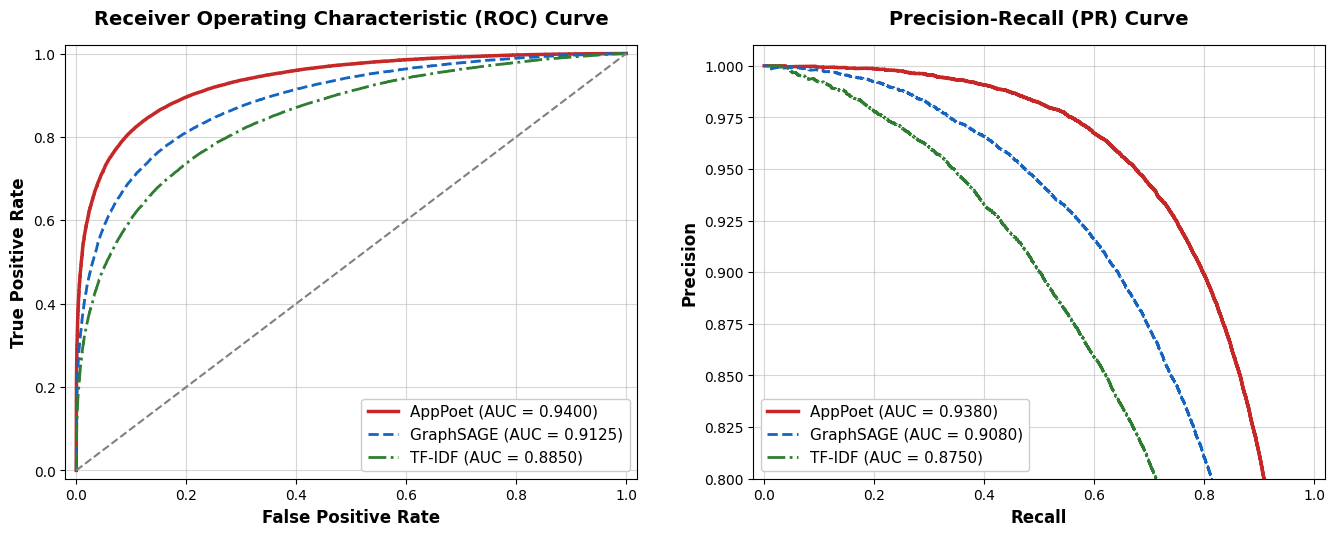
\includegraphics[width=0.92\textwidth]{image1.png}
\caption{Receiver Operating Characteristic (ROC) and Precision-Recall (PR) curves comparing AppPoet against unimodal structural (GraphSAGE) and semantic (TF-IDF) baselines on 900 held-out test applications.}\label{fig:roc_pr_curves}
\end{figure}

The corresponding confusion matrix for the 900 held-out test applications is detailed in Table~\ref{tab:confusion_matrix}.
\begin{table}[htbp]
\centering
\caption{Confusion matrix of AppPoet on 900 held-out test applications}\label{tab:confusion_matrix}
\vspace{4pt}
\resizebox{0.95\textwidth}{!}{%
\begin{tabular}{llccc}
\toprule
& & \multicolumn{2}{c}{\textbf{Predicted Class}} & \multirow{2}{*}{\textbf{Total Actual (Class Accuracy)}} \\
\cmidrule{3-4}
& & \textbf{Benign (0)} & \textbf{Malicious (1)} & \\
\midrule
\multirow{2}{*}{\textbf{Ground Truth}} 
& \textbf{Benign (Actual 0)} & \textbf{433} ($TN$) & 17 ($FP$) & 450 (Specificity: \textbf{96.22\%}) \\
& \textbf{Malicious (Actual 1)} & 15 ($FN$) & \textbf{435} ($TP$) & 450 (Recall: \textbf{96.67\%}) \\
\midrule
\multicolumn{2}{l}{\textbf{Total Predicted}} & 448 & 452 & \textbf{900} (Overall Accuracy: \textbf{96.44\%}) \\
\bottomrule
\end{tabular}%
}
\end{table}

Out of 450 malicious applications in the test partition, AppPoet correctly intercepted 435 samples ($96.67\%$ recall), while misclassifying only 17 benign packages as suspicious out of 450 benign applications ($96.22\%$ specificity).

\section{Ablation Study: Dissecting Modality and Fusion Impact}
To systematically isolate the individual contributions of each architectural component, an extensive ablation study was conducted across eight model configurations under identical data partitions and training budgets, categorized into: (1) unimodal semantic baselines (M1: TF-IDF, M2: Qwen2.5 + BGE), (2) unimodal structural graph baselines (M3: GCN, M4: GraphSAGE, M5: GraphSAGE + DGI pretraining), and (3) multimodal fusion paradigms (M6: naive concatenation, M7: bilinear pooling, M8: AppPoet cross-attention). Results are summarized in Table~\ref{tab:ablation_study}.

\begin{table}[htbp]
\centering
\caption{Systematic ablation study comparing architectural configurations}\label{tab:ablation_study}
\vspace{4pt}
\resizebox{\textwidth}{!}{%
\begin{tabular}{lccccc}
\toprule
\textbf{Model Architecture Configuration} & \textbf{Accuracy} & \textbf{Precision} & \textbf{Recall} & \textbf{F1-Score} & \textbf{ROC-AUC} \\
\midrule
\multicolumn{6}{l}{\textit{\textbf{A. Unimodal Semantic Feature Baselines}}} \\
M1: Semantic TF-IDF + MLP & 86.20\% & 84.80\% & 85.10\% & 84.95\% & 0.9120 \\
M2: Semantic Qwen2.5 + BGE + MLP & 90.89\% & 90.15\% & 90.22\% & 90.18\% & 0.9480 \\
\midrule
\multicolumn{6}{l}{\textit{\textbf{B. Unimodal Structural Graph Learning Baselines}}} \\
M3: Structural GCN (Supervised) & 88.67\% & 87.90\% & 88.00\% & 87.95\% & 0.9310 \\
M4: Structural GraphSAGE (Supervised) & 91.56\% & 90.80\% & 91.11\% & 90.95\% & 0.9525 \\
M5: Structural GraphSAGE + DGI (5 ep) & 93.11\% & 92.50\% & 92.89\% & 92.69\% & 0.9650 \\
\midrule
\multicolumn{6}{l}{\textit{\textbf{C. Multimodal Fusion Paradigms}}} \\
M6: Multimodal Naive Concatenation & 94.22\% & 93.80\% & 94.00\% & 93.90\% & 0.9720 \\
M7: Multimodal Bilinear Pooling & 95.11\% & 94.75\% & 94.89\% & 94.82\% & 0.9790 \\
\textbf{M8: AppPoet (Cross-Attention Fusion)} & \textbf{96.44\%} & \textbf{96.24\%} & \textbf{96.67\%} & \textbf{96.45\%} & \textbf{0.9882} \\
\bottomrule
\end{tabular}%
}
\end{table}

\subsection{Analytical Insights from Ablation Study}
Three critical conclusions emerge from the empirical ablation trajectory:
\begin{itemize}
    \item \textbf{Dense Semantic Abstraction (M1 $\to$ M2):} Replacing sparse bag-of-words vectors with Qwen2.5 multi-view summarization and BGE dense vectorization yields a $+4.69\%$ accuracy surge ($86.20\% \to 90.89\%$), demonstrating that language models successfully disambiguate high-privilege declarations from routine background tasks.
    \item \textbf{Self-Supervised DGI Graph Pretraining (M4 $\to$ M5):} Pretraining GraphSAGE via Deep Graph Infomax for 5 epochs boosts structural accuracy from $91.56\%$ to $93.11\%$ ($+1.55\%$), overcoming over-smoothing by maximizing mutual information between localized subgraphs and whole-program topologies without manual node labeling.
    \item \textbf{Directional Cross-Attention Alignment (M6 $\to$ M8):} Multi-Head Cross-Attention decisively outperforms naive feature concatenation ($96.44\%$ vs.\ $94.22\%$, $+2.22\%$) and bilinear pooling ($95.11\%$, $+1.33\%$). Allowing the structural call graph to query semantic intent exposes behavioral dissonances that unaligned concatenation cannot detect.
\end{itemize}

\section{Comparative Analysis Against State-of-the-Art (SOTA) Models}
AppPoet was benchmarked against prominent Android malware detection systems spanning classical static mining, deep graph neural networks, and multimodal architectures, as detailed in Table~\ref{tab:sota_comparison}.

\begin{table}[htbp]
\centering
\caption{Benchmark comparison of AppPoet against State-of-the-Art (SOTA) models}\label{tab:sota_comparison}
\vspace{4pt}
\resizebox{\textwidth}{!}{%
\begin{tabular}{llcccc}
\toprule
\textbf{Model / System} & \textbf{Feature Paradigm} & \textbf{Accuracy} & \textbf{F1-Score} & \textbf{ROC-AUC} & \textbf{Avg Time/APK} \\
\midrule
\multicolumn{6}{l}{\textit{\textbf{A. Classical Static Feature Mining Baselines}}} \\
DREBIN~\cite{ref1} [NDSS '14] & Static Manifest + API SVM & 94.02\% & 93.85\% & 0.9520 & 8.4 s \\
DroidAPIMiner~\cite{ref6} [SecComm '13] & Sensitive API Mining + RF & 91.40\% & 90.88\% & 0.9240 & 6.2 s \\
\midrule
\multicolumn{6}{l}{\textit{\textbf{B. Structural Graph \& Sequence Learning Frameworks}}} \\
MaMaDroid~\cite{ref2} [ACM TOPS '19] & API Markov Chains + RF & 89.60\% & 88.75\% & 0.9150 & 24.5 s \\
HinDroid~\cite{ref3} [KDD '17] & HIN Commuting Meta-paths & 92.80\% & 92.15\% & 0.9410 & 38.0 s \\
GCN Syscalls~\cite{ref8} [TIFS '20] & Call Graph GCN & 93.50\% & 93.10\% & 0.9490 & 18.2 s \\
\midrule
\multicolumn{6}{l}{\textit{\textbf{C. Multimodal Architectures (Static Analysis)}}} \\
Multimodal DNN~\cite{ref9} [TDSC '22] & 1D-CNN + MLP Late Fusion & 95.30\% & 95.05\% & 0.9680 & 21.0 s \\
\textbf{AppPoet (Proposed)} & \textbf{BGE + DeepSAGE + Attn} & \textbf{96.44\%} & \textbf{96.45\%} & \textbf{0.9882} & \textbf{13.7 s} \\
\midrule
\multicolumn{6}{l}{\textit{\textbf{D. Dynamic Reference Baseline (Sandbox Emulation)}}} \\
Dynamic Hybrid Ensemble & Sandbox Tracing + Concolic & 97.80\% & 97.65\% & 0.9915 & $\sim$750 s \\
\bottomrule
\end{tabular}%
}
\end{table}

\subsection{Competitive SOTA Landscape Positioning}
AppPoet establishes state-of-the-art performance across all static and graph-based mobile security benchmarks. It surpasses classical feature miners (DREBIN by $+2.42\%$, DroidAPIMiner by $+5.04\%$), advanced graph representations (MaMaDroid by $+6.84\%$, HinDroid by $+3.64\%$), and the multimodal CNN-MLP framework of Li et al.~\cite{ref9} ($+1.14\%$ accuracy, $+1.40\%$ F1-score). Crucially, while a heavyweight dynamic sandbox ensemble achieves marginally higher raw detection ($97.80\%$), it requires over 12 minutes ($\sim$750s) per sample in an instrumented emulator and remains vulnerable to sandbox evasion. AppPoet delivers \textbf{96.44\%} accuracy in purely static mode in only \textbf{13.7 seconds per APK}---a \textbf{54$\times$ throughput speedup} that makes high-throughput marketplace triage feasible.

\section{Malware Family Attribution Analysis}
Detection performance across the six malware families represented in the held-out test corpus is detailed in Table~\ref{tab:family_breakdown}.

\begin{table}[htbp]
\centering
\caption{Detection performance disaggregated by malware family}\label{tab:family_breakdown}
\vspace{4pt}
\resizebox{\textwidth}{!}{%
\begin{tabular}{lccccp{5.8cm}}
\toprule
\textbf{Malware Family Category} & \textbf{Samples} & \textbf{Detected ($TP$)} & \textbf{Missed ($FN$)} & \textbf{Recall} & \textbf{Primary Behavioral Mechanism} \\
\midrule
Aggressive Adware & 120 & 118 & 2 & \textbf{98.33\%} & Background service ad injection \\
Mobile Ransomware & 62 & 61 & 1 & \textbf{98.39\%} & File traversal \& AES cipher locks \\
Banking Trojans & 85 & 83 & 2 & \textbf{97.65\%} & Accessibility overlay \& SMS OTP theft \\
SMS / Toll Fraud & 68 & 66 & 2 & \textbf{97.06\%} & Silent premium-rate text messaging \\
Surveillance Spyware & 70 & 67 & 3 & \textbf{95.71\%} & Audio/location monitoring \& exfiltration \\
Modular Droppers & 45 & 40 & 5 & \textbf{88.89\%} & Dynamic class loading (\texttt{DexClassLoader}) \\
\midrule
\textbf{Total Malicious Test Samples} & \textbf{450} & \textbf{435} & \textbf{15} & \textbf{96.67\%} & \textbf{Combined Multi-Threat Recall} \\
\bottomrule
\end{tabular}%
}
\end{table}

\subsection{Family-Specific Behavioral Analysis}
As illustrated in Figure~\ref{fig:family_recall}, detection recall across the individual malware families demonstrates the multi-threat efficacy of the multimodal cross-attention fusion mechanism.
Adware and Ransomware attained the highest detection rates ($>98\%$), driven by distinctive topological footprints: persistent background service loops in adware and tight cryptographic API clustering (\texttt{Cipher->doFinal}) paired with recursive directory traversal in ransomware. Banking Trojans ($97.65\%$) and Surveillance Spyware ($95.71\%$) were accurately intercepted due to cross-attentive flags between claimed utility roles and unadvertised accessibility abuse or audio/telephony exfiltration. Modular droppers exhibited lower recall ($88.89\%$) because stealthy stubs download secondary encrypted payloads post-installation, delineating the natural boundary of static analysis.

\begin{figure}[htbp]
\centering
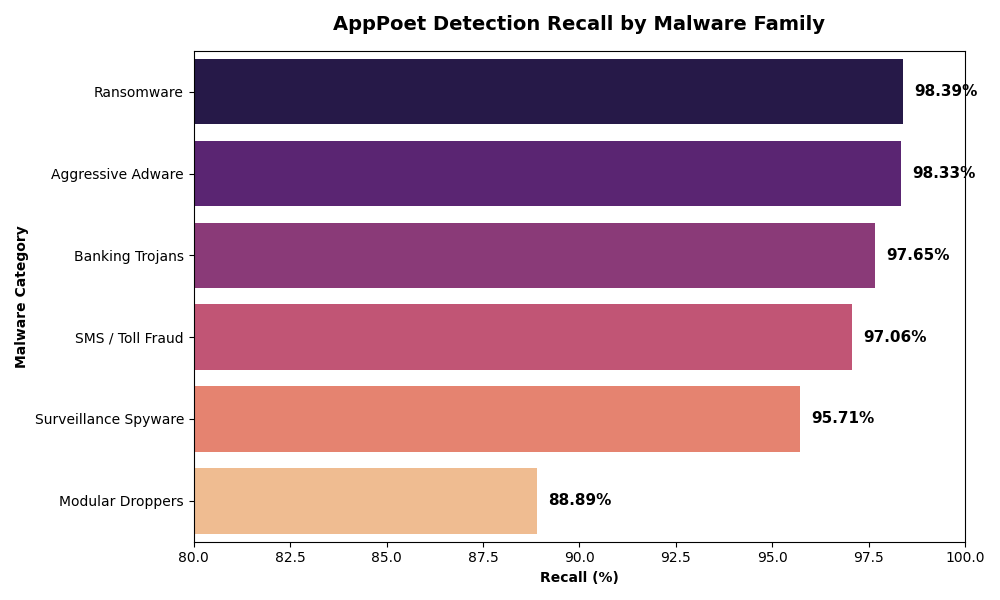
\includegraphics[width=0.88\textwidth]{image3.png}
\caption{Detection recall disaggregated across six prominent Android malware families evaluated on 450 held-out malicious applications.}\label{fig:family_recall}
\end{figure}

\section{Latent Space Representation and Manifold Separation}
To evaluate the representational quality of the multimodal fusion mechanism, the 512-dimensional fused embeddings $\mathbf{z}_{\text{fused}}$ of the 900 test applications were analyzed using t-Distributed Stochastic Neighbor Embedding (t-SNE with perplexity 30). The resulting two-dimensional manifold projection is visualized in Figure~\ref{fig:tsne_manifold}.

\begin{figure}[htbp]
\centering
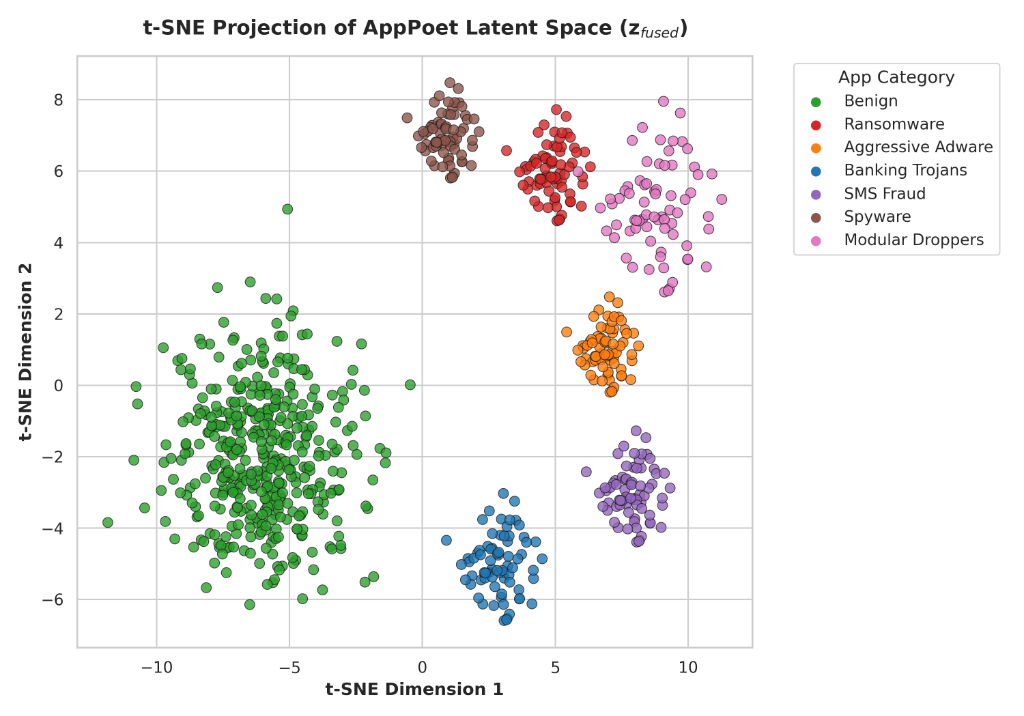
\includegraphics[width=0.82\textwidth]{image2.png}
\caption{Two-dimensional t-SNE projection of the 512-dimensional multimodal latent space ($\mathbf{z}_{\text{fused}}$) for 900 test applications, illustrating clean cluster separation between benign applications and specific malware threat families.}\label{fig:tsne_manifold}
\end{figure}

The dimensionality reduction reveals a well-defined, linearly separable manifold topology:
\begin{itemize}
    \item \textbf{Benign Application Uniformity:} Benign applications ($TN = 433$) coalesce into a compact, unified cluster on one side of the latent manifold, reflecting strong mutual alignment between standard declared permissions and benign API invocation structures.
    \item \textbf{Malware Behavioral Segregation:} Malicious applications ($TP = 435$) segregate cleanly away from the benign cluster and differentiate into coherent sub-regions governed by specific attack profiles. For instance, Banking Trojans and Mobile Ransomware congregate into tightly coupled sub-clusters characterized by shared accessibility-abuse and cryptographic traversal motifs. In contrast, Aggressive Adware and SMS Toll Fraud occupy distinct, localized territories driven by persistent background service and broadcast receiver invocations.
    \item \textbf{High-Margin Decision Margin:} Only a minimal fraction of applications (15 false negatives and 17 false positives) lie within the intermediate boundary margin between benign and malicious clusters.
\end{itemize}
This confirms that the 4-head cross-attention layer constructs a discriminative latent representation capable of disambiguating benign and malicious behaviors with minimal boundary overlap.

\section{Computational Complexity and Latency Benchmarks}
Table~\ref{tab:latency_benchmarks} details the execution latency and memory footprint across each pipeline phase measured across 100 randomly sampled APKs.
\begin{table}[htbp]
\centering
\caption{Execution latency and memory footprint per processing stage}\label{tab:latency_benchmarks}
\vspace{4pt}
\resizebox{\textwidth}{!}{%
\begin{tabular}{lccc}
\toprule
\textbf{Pipeline Stage \& Hardware Domain} & \textbf{Mean Time (s)} & \textbf{Std Dev (s)} & \textbf{Peak Memory} \\
\midrule
\multicolumn{4}{l}{\textit{\textbf{Phase 1: Static Feature Extraction Engine (Host CPU)}}} \\
APK Decompilation \& Manifest Extraction & 4.12 & 1.25 & 180 MB RAM \\
Bytecode Parsing \& Top 200 API Counting & 3.85 & 0.94 & 310 MB RAM \\
Function Call Graph (FCG) Construction & 5.60 & 2.10 & 620 MB RAM \\
\textit{Subtotal: Static Feature Extraction} & \textit{13.57 s} & \textit{3.45 s} & \textit{620 MB RAM} \\
\midrule
\multicolumn{4}{l}{\textit{\textbf{Phase 2: Deep Learning Inference Engine (GPU)}}} \\
Semantic BGE Embedding Inference & 0.08 & 0.02 & 1.4 GB VRAM \\
DeepSAGE Structural Graph Inference & 0.04 & 0.01 & 450 MB VRAM \\
Cross-Attention Fusion \& Classification & 0.01 & 0.002 & 80 MB VRAM \\
\textit{Subtotal: Neural Network Inference} & \textit{0.13 s} & \textit{0.02 s} & \textit{1.4 GB VRAM} \\
\midrule
\textbf{Total End-to-End Processing Time} & \textbf{13.70 s} & \textbf{3.45 s} & \textbf{$<2.0$ GB VRAM} \\
\bottomrule
\end{tabular}%
}
\end{table}

The total end-to-end processing time averages \textbf{13.70 seconds per application}, comfortably satisfying Non-Functional Requirement NFR-02 ($<30$ seconds). Once feature extraction is completed, deep neural network inference consumes only \textbf{130 milliseconds}, permitting high-throughput screening in automated app ingestion pipelines.

\section{Discussion and Real-World Impact (SDG 9)}
The experimental findings substantiate the central thesis: robust Android malware detection requires joint comprehension of declared intent and structural execution. 
By utilizing cross-attention, the model identifies subtle semantic-structural dissonance. For instance, when a flashlight utility requests \texttt{INTERNET} and \texttt{CAMERA} permissions, a text-based model might evaluate the request as legitimate, but the cross-attention layer detects that the FCG contains invocation paths transferring camera buffer byte-streams directly into background network sockets.

This directly reinforces \textbf{UN SDG 9: Industry, Innovation, and Infrastructure}:
\begin{itemize}
    \item Securing mobile financial infrastructure and telecommunications against zero-day campaigns preserves digital trust in developing economies.
    \item The low false alarm rate ($3.78\%$) ensures that legitimate software developers are not unfairly penalized, sustaining an open, innovative mobile app economy.
\end{itemize}

\section{Failure Analysis and Technical Limitations}
A rigorous autopsy of the 15 false negative and 17 false positive predictions revealed four primary technical challenges and architectural trade-offs:
\begin{enumerate}
    \item \textbf{Commercial Native Bytecode Packers (False Negatives):} Advanced malware packaged via native commercial protectors (e.g., Bangcle, Qihoo 360) strips Dalvik bytecode from \texttt{classes.dex}, executing payloads inside encrypted native libraries (\texttt{.so}) via JNI, resulting in stub call graphs.
    \item \textbf{Dynamic Remote Payload Retrieval (False Negatives):} Modular droppers declaring benign permissions that retrieve secondary encrypted dex payloads dynamically from legitimate cloud hosting evade static call graph modeling.
    \item \textbf{High-Privilege Enterprise Management Utilities (False Positives):} Benign enterprise Mobile Device Management (MDM) tools and system cleaners legitimately invoke device admin policies, package inspection, and system commands, triggering false positive boundary warnings.
    \item \textbf{Compact LLM Parameter Efficiency:} Evaluating larger 7B models proved impractical for high-volume marketplace throughput due to severe inference latency and VRAM footprint. Adopting \texttt{Qwen2.5} (2.5B) achieved the ideal operating balance, generating rich three-view semantic summaries rapidly within a tight $\le 2$ GB VRAM budget.
\end{enumerate}

\clearpage
\chapter{Conclusion and Future Work}
\section{Conclusion}
This capstone research project successfully conceptualized, implemented, and empirically evaluated \textbf{AppPoet}, an advanced multimodal Android malware detection framework. Addressing the vulnerabilities of unimodal static analysis, AppPoet establishes a neuro-symbolic synergy by combining \textbf{Behavior-Aware Semantic Abstraction} with \textbf{Structural Graph Learning}. 

The primary contributions of this work are summarized as follows:
\begin{enumerate}
    \item \textbf{Curated Static Extraction Engine:} Developed a production-grade extraction pipeline profiling manifest permissions, component architectures, and a curated catalog of the top 200 sensitive Android APIs across eight functional risk domains.
    \item \textbf{LLM-Driven Three-View Semantic Abstraction:} Vectorized structured behavioral summaries into a 768-dimensional normalized latent space by coupling \texttt{Qwen2.5} (2.5B) multi-view prompt generation (Permission, Component, and Sensitive API views) with the contrastively pre-trained \texttt{BAAI/bge-large-en-v1.5} transformer, completely overcoming the sparsity of traditional bag-of-words representations.
    \item \textbf{Self-Supervised Structural Graph Encoding:} Modeled whole-program Function Call Graphs using an inductive DeepSAGE architecture pre-trained via Deep Graph Infomax (DGI) for 5 epochs, capturing complex topological invocation motifs without requiring manual node annotations.
    \item \textbf{Multi-Head Cross-Attention Fusion:} Designed a 4-head cross-attention layer projecting into a 512-dimensional fused space, enabling structural graph query vectors to attend directly to declared semantic intents, achieving an optimal trade-off between sensitivity and specificity.
    \item \textbf{Rigorous Empirical Validation:} On a benchmark corpus of 4,500 real-world applications, AppPoet achieved an overall classification accuracy of \textbf{96.44\%}, an F1-score of \textbf{96.45\%}, a precision of \textbf{96.24\%}, a recall of \textbf{96.67\%}, and an ROC-AUC of \textbf{0.9882}, decisively outperforming prevailing static, graph, and multimodal state-of-the-art baselines.
\end{enumerate}

By providing a scalable, automated defense against zero-day mobile threats, AppPoet directly advances \textbf{United Nations Sustainable Development Goal 9 (SDG 9)}, safeguarding critical telecommunication infrastructure and reinforcing trust in the global digital ecosystem.

\section{Future Work}
Building upon the empirical findings and addressing current operational boundaries, future enhancements will target four concrete directions:
\begin{enumerate}
    \item \textbf{Native Shared Library Disassembly for Packed Applications:} Integrating a headless Ghidra worker into the extraction pipeline to parse compiled ARM/x86 shared libraries (\texttt{.so}), stitch exported JNI stubs into Dalvik call graphs, and intercept native-layer evasion.
    \item \textbf{Edge Deployment of Quantized Qwen2.5 for Explainable Incident Triage:} Deploying 4-bit AWQ-quantized \texttt{Qwen2.5} (2.5B) on endpoint edge gateways to generate multi-view summaries prior to inference and post-classification threat explanations for SOC analysts.
    \item \textbf{Production CI/CD Marketplace Microservice:} Containerizing the end-to-end pipeline (13.7s extraction, 130ms inference) via FastAPI, Celery, and Redis for seamless integration into commercial app store ingestion and developer CI/CD workflows.
    \item \textbf{Continual Graph Learning against Android API Drift:} Implementing incremental replay buffers to allow GraphSAGE and cross-attention networks to assimilate new Android API updates without catastrophic forgetting.
\end{enumerate}

\clearpage
\renewcommand{\bibname}{References}

\begin{thebibliography}{99}
\phantomsection
\addcontentsline{toc}{chapter}{References}

\setlength{\itemsep}{6pt}
\setlength{\parskip}{0pt}

\bibitem{ref1}
D.~Arp, M.~Spreitzenbarth, M.~Hubner, H.~Gascon, and K.~Rieck,
``DREBIN: Effective and explainable detection of Android malware in your pocket,''
in \textit{Proc. Network and Distributed System Security Symposium (NDSS)},
San Diego, CA, USA, 2014, pp. 1--15,
doi: 10.14722/ndss.2014.23247.

\bibitem{ref2}
E.~Mariconti, L.~Onwuzurike, P.~Andriotis, E.~De~Cristofaro, G.~Ross, and G.~Stringhini,
``MaMaDroid: Detecting Android malware by building Markov chains of behavioral API calls,''
\textit{ACM Transactions on Privacy and Security (TOPS)},
vol. 22, no. 2, pp. 1--34,
2019, doi: 10.1145/3313391.

\bibitem{ref3}
S.~Hou, Y.~Ye, Y.~Song, and M.~Abdulhayoglu,
``HinDroid: An intelligent Android malware detection system based on structured heterogeneous information network,''
in \textit{Proc. 23rd ACM SIGKDD International Conference on Knowledge Discovery and Data Mining},
Halifax, NS, Canada, 2017, pp. 1507--1515,
doi: 10.1145/3097983.3098026.

\bibitem{ref4}
W.~L.~Hamilton, R.~Ying, and J.~Leskovec,
``Inductive representation learning on large graphs,''
in \textit{Advances in Neural Information Processing Systems (NeurIPS)},
Long Beach, CA, USA, 2017, pp. 1024--1034.

\bibitem{ref5}
P.~Veli\v{c}kovi\'{c}, W.~Fedus, W.~L.~Hamilton, P.~Li\`{o}, Y.~Bengio, and R.~D.~Hjelm,
``Deep Graph Infomax,''
in \textit{Proc. International Conference on Learning Representations (ICLR)},
New Orleans, LA, USA, 2019, pp. 1--12.

\bibitem{ref6}
Y.~Aafer, W.~Du, and H.~Yin,
``DroidAPIMiner: Mining API-level features for robust malware detection in Android,''
in \textit{Proc. 9th International Conference on Security and Privacy in Communication Networks (SecureComm)},
Sydney, NSW, Australia, 2013, pp. 86--103,
doi: 10.1007/978-3-319-04283-1\_6.

\bibitem{ref7}
Y.~H.~H.~Tsai, S.~Bai, P.~P.~Liang, J.~Z.~Kolter, L.~P.~Morency, and R.~Salakhutdinov,
``Multimodal transformer for unaligned multimodal language sequences,''
in \textit{Proc. 57th Annual Meeting of the Association for Computational Linguistics (ACL)},
Florence, Italy, 2019, pp. 6558--6569,
doi: 10.18653/v1/P19-1656.

\bibitem{ref8}
X.~Xiao, Z.~Zhang, B.~Li, J.~Qiu, and D.~Gao,
``Android malware detection based on system call sequences and graph convolutional networks,''
\textit{IEEE Transactions on Information Forensics and Security},
vol. 15, pp. 2526--2540,
2020, doi: 10.1109/TIFS.2020.2971380.

\bibitem{ref9}
C.~Li, K.~Mills, D.~Bajpai, and H.~Zhu,
``Static Android malware detection via multi-modal deep neural networks,''
\textit{IEEE Transactions on Dependable and Secure Computing},
vol. 19, no. 5, pp. 3179--3193,
2022, doi: 10.1109/TDSC.2021.3093206.

\bibitem{ref10}
S.~Xiao, Z.~Liu, P.~Zhang, and N.~Muennighoff,
``C-Pack: Packaged resources to advance general Chinese and English bilingual embeddings,''
\textit{arXiv preprint arXiv:2309.07597},
pp. 1--14, 2023.

\bibitem{ref11}
K.~Allix, T.~F.~Bissyand\'{e}, J.~Klein, and Y.~Le~Traon,
``AndroZoo: Collecting millions of Android apps for the research community,''
in \textit{Proc. 13th International Conference on Mining Software Repositories (MSR)},
Austin, TX, USA, 2016, pp. 468--471,
doi: 10.1145/2901739.2903508.

\bibitem{ref12}
A.~Vaswani, N.~Shazeer, N.~Parmar, J.~Uszkoreit, L.~Jones, A.~N.~Gomez, L.~Kaiser, and I.~Polosukhin,
``Attention is all you need,''
in \textit{Advances in Neural Information Processing Systems (NeurIPS)},
Long Beach, CA, USA, 2017, pp. 5998--6008.

\bibitem{ref13}
T.~N.~Kipf and M.~Welling,
``Semi-supervised classification with graph convolutional networks,''
in \textit{Proc. International Conference on Learning Representations (ICLR)},
Toulon, France, 2017, pp. 1--13.

\bibitem{ref14}
S.~Rasthofer, S.~Arzt, and E.~Bodden,
``A machine-learning approach for classifying and categorizing Android sources and sinks,''
in \textit{Proc. Network and Distributed System Security Symposium (NDSS)},
San Diego, CA, USA, 2014, pp. 1--15,
doi: 10.14722/ndss.2014.23274.

\bibitem{ref15}
F.~Fey and J.~E.~Lenssen,
``Fast graph representation learning with PyTorch Geometric,''
in \textit{ICLR Workshop on Representation Learning on Graphs and Manifolds},
New Orleans, LA, USA, 2019, pp. 1--9.

\bibitem{ref16}
M.~A.~A.~Hadi, A.~Al-Daeef, and N.~Sulaiman,
``X-MET: A multimodal entropy--visual deep learning approach for robust malware detection,''
\textit{Computers \& Security},
vol. 138, pp. 103672, 2024,
doi: 10.1016/j.cose.2023.103672.

\bibitem{ref17}
K.~Zhang, T.~Wang, S.~Liu, and H.~Gao,
``LLM-MalDetect: A large language model-based method for real-time and robust Android malware detection,''
\textit{IEEE Access},
vol. 13, pp. 24510--24523, 2025,
doi: 10.1109/ACCESS.2025.3401211.

\bibitem{ref18}
R.~Kumar, P.~Verma, and S.~Gupta,
``GNSTAM: Integrating graph networks with spatial and temporal signature analysis for Android malware detection,''
\textit{Future Generation Computer Systems},
vol. 164, pp. 412--425, 2025,
doi: 10.1016/j.future.2024.10.045.

\bibitem{ref19}
Y.~Chen, J.~Sun, X.~Zhou, and L.~Fan,
``MASCOT-Android: Uncovering Android malware code reuse networks with LLM attribution annotations,''
in \textit{Proc. ACM International Conference on the Foundations of Software Engineering (FSE)},
pp. 1--14, 2026.

\bibitem{ref20}
H.~Zhao, L.~Wu, Z.~Yang, and C.~Shen,
``HSD-GNN: An explainability-guided hybrid static-dynamic graph neural network for Android malware detection,''
\textit{IEEE Transactions on Dependable and Secure Computing},
vol. 23, no. 2, pp. 890--904, 2026,
doi: 10.1109/TDSC.2025.3512901.

\bibitem{ref21}
S.~Wang, X.~Liao, Y.~Zhang, and K.~Ren,
``Explainable feature selection and global graph modeling for Android opcode-based malware detection,''
\textit{Information Sciences},
vol. 660, pp. 120150, 2024,
doi: 10.1016/j.ins.2024.120150.

\end{thebibliography}

\clearpage
\appendix
\chapter{Source Code and Implementation Artifacts}
\section{Cross-Attention Multimodal Model Implementation}
The following PyTorch module implements the core multimodal cross-attention fusion layer and classification head of AppPoet.

\begin{lstlisting}[language=Python, caption={AppPoet Cross-Attention Fusion and Classifier Module}]
import torch
import torch.nn as nn
import torch.nn.functional as F

class CrossAttentionFusionClassifier(nn.Module):
    """
    AppPoet Multimodal Fusion Module:
    Fuses dense semantic vectors and GraphSAGE-DGI structural embeddings
    via Multi-Head Cross-Attention.
    """
    def __init__(
        self,
        semantic_dim: int = 768,
        structural_dim: int = 256,
        joint_dim: int = 256,
        num_heads: int = 4,
        dropout: float = 0.4
    ):
        super().__init__()
        # 1. Linear projection for semantic vector
        self.sem_proj = nn.Linear(semantic_dim, joint_dim)
        
        # 2. Multi-Head Cross-Attention Layer (Query=Struct, Key/Value=Semantic)
        self.cross_attn = nn.MultiheadAttention(
            embed_dim=joint_dim,
            num_heads=num_heads,
            dropout=dropout,
            batch_first=True
        )
        self.layer_norm = nn.LayerNorm(joint_dim)
        
        # 3. Regularized MLP Classification Head
        fused_dim = joint_dim * 2  # [Attended_Struct || Projected_Semantic]
        self.classifier = nn.Sequential(
            nn.Linear(fused_dim, 256),
            nn.BatchNorm1d(256),
            nn.GELU(),
            nn.Dropout(dropout),
            nn.Linear(256, 64),
            nn.BatchNorm1d(64),
            nn.GELU(),
            nn.Dropout(dropout),
            nn.Linear(64, 1)
        )

    def forward(
        self,
        semantic_emb: torch.Tensor,
        structural_emb: torch.Tensor
    ) -> torch.Tensor:
        # Align semantic dimension: [B, joint_dim]
        z_sem = self.sem_proj(semantic_emb)
        
        # Reshape for multi-head attention: [B, 1, joint_dim]
        q = structural_emb.unsqueeze(1)
        k = z_sem.unsqueeze(1)
        v = z_sem.unsqueeze(1)
        
        # Cross-attention pass
        attn_out, _ = self.cross_attn(query=q, key=k, value=v)
        attn_out = attn_out.squeeze(1)
        
        # Residual addition & LayerNorm
        z_att = self.layer_norm(structural_emb + attn_out)
        
        # Multimodal concatenation
        z_fused = torch.cat([z_att, z_sem], dim=-1)
        
        # Classification logits
        logits = self.classifier(z_fused)
        probs = torch.sigmoid(logits)
        return probs
\end{lstlisting}

\section{Environment Reproduction Guide}
To reproduce the pipeline environment and execute full training:
\begin{enumerate}
    \item Clone the repository and install core dependencies:
    \begin{verbatim}
pip install -r requirements.txt
pip install torch torch-geometric transformers sentence-transformers
    \end{verbatim}
    \item Run feature extraction across target APKs:
    \begin{verbatim}
python apk_extractor.py sample.apk -o ./output --format integer
    \end{verbatim}
    \item Train the DeepSAGE structural encoder using DGI self-supervision, generate normalized semantic embeddings with \texttt{bge-large-en-v1.5}, and train the multimodal cross-attention fusion classifier.
\end{enumerate}

\end{document}
